\chapter{Funzioni in $\mathbb{R}^n$}

\section{Limiti di funzioni}

Sia una funzione
\begin{align}
f \, : \, A\subseteq \mathbb{R}^n {}&\longrightarrow \mathbb{R}^m \quad n,m\geq 1\\
\underline{x}=(x_1,\dots,x_n) &\longrightarrow \underline{f}(\underline{x})=(f_1(\underline{x}), \dots , f_n(\underline{x})) \nonumber
\end{align}
e sia $\underline{x}^0 \in acc(A)$, avremo
\begin{align}
\underset{\underline{x} \rightarrow \underline{x}^0}{\lim}\,\underline{f}(\underline{x})=\underline{l}=(l_1,\dots,l_n)\in \mathbb{R}^m
\end{align}
Ma questo implica che
\begin{align}
\underset{x_i\rightarrow x_i^0}{\lim} f_i(x_i)=l_i \quad \forall i =1,\dots,n
\end{align}
e quindi il problema si riduce allo studio dei limiti $l_i \in \mathbb{R}$

\subsection{Limiti in $\mathbb{R}$}

Siano $\underline{f} \, : \, A\subseteq \mathbb{R}^n \longrightarrow \mathbb{R}$ e $\underline{x}^0 \in acc(A)$, si definisce il \textbf{limite} di $\underline{f}$ ad $\underline{x}^0$ come:
\begin{align}
{}&\underset{\underline{x}\rightarrow\underline{x}^0}{\lim}f(\underline{x})=l \in \mathbb{R}\cup \left\{\pm \infty \right\}\\ 
&\updownarrow \nonumber \\ 
&\forall U(l) \; \exists I_\delta(\underline{x}^0) \, : \, f(\underline{x}) \in U(l) \quad \forall \underline{x}\in I_\delta(\underline{x}^0)\backslash\left\{\underline{x}^0\right\}\\ 
&\updownarrow \nonumber \\ 
&\forall \epsilon>0 \, \exists \delta_\epsilon \, : \, |f(\underline{x}) - l|_1<\epsilon \quad \forall \underline{x}\in A \, : \, |\underline{x} - \underline{x}^0|_n\leq \delta_\epsilon
\end{align}

\textbf{Nota bene:} Tutti i teoremi per i limiti validi in $\mathbb{R}$ lo sono anche per $\mathbb{R}^n$.

\section{Funzioni continue in $\mathbb{R}^n$}

Si parla di \textbf{continuità in un punto} $\underline{x}^0\in A$ quando 
\begin{align}
\exists \underset{\underline{x}\rightarrow\underline{x}^0}{\lim} \, f(\underline{x})= f(\underline{x}^0)
\end{align} 
e di \textbf{continuità in tutto l'insieme} $A$ quando vale $\forall x\in A$.

\subsection{Connessione}

Si dice che un insieme $A$ è connesso se $\nexists A_1,A_2$ tali che
\begin{enumerate}
	\item $A_1\neq \emptyset \neq A_2$
	\item $A_1\cap A_2=\emptyset$
	\item $A= A_1\cup A_2$
\end{enumerate}

\subsection{Teoremi sulle funzioni continue}

Enunciamo senza dimostrazione alcuni teoremi utili sulle funzioni continue:
\begin{enumerate}
	\item \textbf{Primo teorema:}
	
	\textit{$f$ è continua se e solo se $\forall \underset{aperto}{E} \in \mathbb{R}$ si ha che $f^{-1}(E)$ è aperto}
	
	\item \textbf{Teorema di Weierstrass:}
	
	\textit{Sia $f$ continua in $D\subset \mathbb{R^n}$ chiuso e limitato (compatto), allora $f$ ammette massimo e minimo in $D$ tali che}
	\begin{align}
	{}&x_m \, : \, f(x_m)=\underset{x\in D}{min}f(x)\leq f(x) \quad \forall x \in D \\
	&x_M \, : \, f(x_M)=\underset{x\in D}{max}f(x)\geq f(x) \quad \forall x \in D
	\end{align}
	
	\item \textbf{Teorema dell'esistenza dei valori intermedi:}
	
	\textit{Siano $f \, : \, D\subset \mathbb{R}^2 \longrightarrow \mathbb{R}$ continua e $D$ chiuso, limitato e connesso.}
	
	\textit{Allora $f$ assume tutti i valori possibili tra il suo massimo e il suo minimo.}
\end{enumerate}

\section{Funzioni in $\mathbb{R}^2$}

Studiamo ora un categoria di funzioni in $\mathbb{R}^n$ molto specifica, le funzioni in $\mathbb{R}^2$, ovvero tali che
\begin{align}
f \, : \, A\subseteq \mathbb{R}^2 {}&\longrightarrow \mathbb{R} \\
(x,y) &\longrightarrow f(x,y) \nonumber
\end{align}

Chiamiamo \textbf{Grafico} di una funzione il seguente insieme:
\begin{align}
\{(x,y,z) \, : \, (x,y)\in D \, ; \, z=f(x,y)\}
\end{align}

E chiamiamo \textbf{curve (o linee) di livello}:
\begin{align}
\{ (x,y) \in D \, : \, f(x,y)=cost. \}
\end{align}

\subsubsection{Esempi di calcolo dell'insieme di definizione}

\begin{enumerate}
	\item $f(x,y)=\sqrt{4-x^2-y^2} \implies D= \{ (x,y) \, : \, x^2 + y^2 \leq 4 \}$
	
	\item $f(x,y)=\ln(4-x^2-y^2) \implies D= \{ (x,y) \, : \, x^2 + y^2 < 4 \}$
\end{enumerate}

\subsubsection{Funzioni radiali}

Sono una categoria di $f\in \mathbb{R}^2$ del tipo

\begin{align}
f(x,y)=f(\sqrt{x^2 + y^2})
\end{align}

che possono essere quindi espresse come funzioni di una sola variabile.

Le linee di livello di queste funzioni possono essere solo circonferenze.

Un esempio di funzione radiale è scritto poco sopra, infatti

 $f(x,y)=\sqrt{4-x^2-y^2} = \sqrt{4-t^2}=f(t=\sqrt{x^2 + y^2})$
 
\newpage
 
\subsection{Calcolo dei limiti}
 
 Iniziamo dando nuovamente la definizione di limite:
  \begin{align}
 {}&\underset{\underline{p}\rightarrow \underline{p}_0}{\lim} f(x,y)=l\in \mathbb{R} \\ 
 &\updownarrow \nonumber\\
 &\forall \epsilon >0 \quad \exists \delta_\epsilon>0 \, : \, |f(x,y)-l|<\epsilon \quad \forall (x_0,y_0) \, : \, d(\underline{p},\underline{p}_0)<\delta_\epsilon \\
 &\left\{
 \begin{array}{cc}
 &\underline{p}=(x,y) \quad ; \quad \underline{p}_0=(x_0,y_0) \\
 &d(\underline{p},\underline{p}_0)=\sqrt{(x-x_0)^2 + (y-y_0)^2}\\
 \end{array} 
 \right.
 \end{align}
 
 Il calcolo dei limiti in più dimensione è una questione molto più complicata rispetto a quelli in una sola. 
 
 Infatti affinché esista un limite, la funzione vi teve tendere da tutte le infinite direzioni e traiettorie possibili! (e quindi non solo dalle rette parallele agli assi, per esempio).
 
 Come procediamo allora?
 
 Innanzitutto dobbiamo trovare un \textbf{candidato limite}, che \underline{potrebbe} (ma \underline{non è detto} che sia) il valore da noi cercato.
 
  Dato un punto $(x_0,y_0)$ possiamo utilizzare due metodi:
 
 \begin{enumerate}
 	\item \textbf{Limite lungo le parallele agli assi}:
 	\begin{align}
 	l_x = \underset{x\rightarrow x_0}{\lim} f(x,y_0) \\
 	l_x = \underset{y\rightarrow y_0}{\lim} f(x_0,y) 
 	\end{align}
 	se $l_x=l_y$ abbiamo un candidato limite valido (ma non è detto sia il limite!), altrimenti possiamo fermarci subito.
 	
 	\item \textbf{Limite lungo una curva $\gamma$:}
 	\begin{align}
 	{}&\underline{r}(t) = \left\{
 	\begin{array}{cc}
 	x=x(t)\\
 	y=y(t)
 	\end{array}
 	\right. 	\quad ; \quad \left\{
 	\begin{array}{cc}
 	x_0=x(t_0)\\
 	y_0=y(t_0)
 	\end{array}
 	\right. \\
 	&\underset{t\rightarrow t_0}{\lim}f(x(t),y(t))=l_\gamma
 	\end{align}
 	
 	Anche qui, se troviamo due curve $\gamma_1$ e $\gamma_2$ tali che $l_{\gamma_1} \neq l_{\gamma_2}$ possiamo interrompere subito la ricerca.
 \end{enumerate}

Vediamo alcuni esempi calcolabili con le scarse conoscenze al momento in nostro possesso:
\begin{enumerate}
	\item $\underset{\underline{p}\rightarrow \underline{p}_0}{\lim} \frac{x^2}{\sqrt{x^2 + y^2}} \quad ; \quad \underline{p}_0=(0,0) \quad ; \quad  x\in A=\mathbb{R}^2\backslash \{\underline{p}_0\}$
	
	\bigskip
	Cerchiamo un candidato limite col primo metodo:
	\begin{align}
	{}&\underset{x\rightarrow x_0}{\lim}f(x,0)= \underset{x\rightarrow x_0}{\lim} \frac{x^2}{\sqrt{x^2}}= \underset{x\rightarrow x_0}{\lim} |x| = 0\\
	&\underset{y\rightarrow y_0}{\lim}f(0,y)= \underset{x\rightarrow x_0}{\lim} \frac{0}{\sqrt{y^2}}= 0
	\end{align}
	
	Abbiamo quindi un candidato in $l=0$.
	
	Applichiamo la definizione di limite:
	\begin{align}
	\left|\frac{x^2}{\sqrt{x^2 + y^2}}-0\right| = \frac{x^2}{\sqrt{x^2 + y^2}}\leq \frac{x^2 + y^2}{\sqrt{x^2 + y^2}}=\sqrt{x^2 + y^2}
	\end{align}
	
	Abbiamo maggiorato $x^2$ con $x^2 + y^2$.
	
	Notiamo come $\sqrt{x^2 + y^2}$ nella def. di limite deve essere $<\delta_\epsilon$, e quindi avremo
	
	\begin{align}
	\left|\frac{x^2}{\sqrt{x^2 + y^2}}-0\right|< \delta_\epsilon=\epsilon \quad \forall (x,y) \, : \, \sqrt{x^2 + y^2}<\delta_\epsilon
	\end{align}
	
	E quindi $0$ è effettivamente il limite.
	
	\item $\underset{\underline{p}\rightarrow \underline{p}_0}{\lim} \frac{x}{\sqrt{x^2 + y^2}} \quad ; \quad \underline{p}_0=(0,0) \quad ; \quad  x\in A=\mathbb{R}^2\backslash \{\underline{p}_0\}$
	
	\bigskip
	In questo caso, procedendo col primo metodo avremo:
	\begin{align}
	{}&\underset{x\rightarrow x_0}{\lim}f(x,0)= \underset{x\rightarrow x_0}{\lim} \frac{x}{\sqrt{x^2}}= \underset{x\rightarrow x_0}{\lim} \frac{1}{|x|} = +\infty\\
	&\underset{y\rightarrow y_0}{\lim}f(0,y)= \underset{x\rightarrow x_0}{\lim} \frac{0}{\sqrt{y^2}}= 0
	\end{align}
	
	E vediamo già che $l_x\neq l_y$ e quindi fermiamo subito la ricerca.
	
	\item $\underset{\underline{p}\rightarrow \underline{p}_0}{\lim} \frac{x-y}{x + y} \quad ; \quad \underline{p}_0=(0,0) \quad ; \quad  x\in A=\mathbb{R}^2\backslash \{x=y\}$
	
	\bigskip
	
	Con il primo metodo troviamo
	\begin{align}
	&\underset{x\rightarrow x_0}{\lim}f(x,0)= \underset{x\rightarrow x_0}{\lim} \frac{x}{x}= +1\\
	&\underset{y\rightarrow y_0}{\lim}f(0,y)= \underset{x\rightarrow x_0}{\lim} \frac{y}{-y}= -1
	\end{align}
	
	e quindi buca, visto che $l_x\neq l_y$
	
	Vediamo come anche col secondo metodo non si abbia limite:
	
	Prendendo tutte le rette possibili con $y=mx$
	\begin{align}
	y=mx \implies f(x,mx)=\frac{x + mx}{x - mx}= \frac{1+m}{1-m}
	\end{align}
	
	Abbiamo qualcosa dipendente da una variabile, e quindi infiniti possibili risultati, mentre il limite deve essere unico per tutte le direzioni.
	
	\item $\underset{\underline{p}\rightarrow \underline{p}_0}{\lim}\frac{x^2 y^2}{x^2 + y^2}  \quad ; \quad \underline{p}_0=(0,0) \quad ; \quad  x\in A=\mathbb{R}^2\backslash \{\underline{p}_0\}$
	
	\bigskip
		
	è evidente come $f(0,y)=0=f(x,0)$ e come
	
	 $f(x,mx)=\frac{m^2 x^2}{1+m^2}\overset{x\rightarrow 0}{\longrightarrow} 0$
	
	E quindi con entrambi i metodi si trova un candidato in $l=0$
	
	Applicando la definizione di limite si trova
	\begin{align}
	0\leq \left|\frac{x^2 y^2}{x^2 + y^2} - 0\right|= \frac{x^2 y^2}{x^2 + y^2}\leq x^2 + y^2 < \delta^2_\epsilon
	\end{align}
	
	E facendo discorsi analoghi all'esempio 2 possiamo dire che $l=0$ è proprio il nostro limite.
\end{enumerate}

\subsubsection{Calcolo dei limiti in forma polare} 

Un comodo metodo per risolvere i limiti è quello di lavorare in coordinate polari nel seguente modo:

\begin{align}
&\left\{
\begin{array}{cc}
x=x_0 + \rho \cos(\theta)\\
y=y_0 + \rho \sin(\theta)
\end{array}
\right. \\
&\downarrow \nonumber \\
&|f(\rho \cos(\theta),\rho \sin(\theta)) - l|<\epsilon \leftrightarrow \rho \in [0,\delta_\epsilon] \quad \forall \theta \in [0,2\pi]
\end{align}
Questo implica anche che
\begin{align}
{}&s(\rho)= \underset{\theta}{sup}|f(\rho \cos(\theta),\rho \sin(\theta)) - l|<\epsilon \leftrightarrow \rho \in [0,\delta_\epsilon] \quad \forall \theta \in [0,2\pi]\\
&s(\rho)\geq 0
\end{align}
E quindi avremo che 
\begin{align}
\underset{\rho \rightarrow 0}{\lim}s(\rho)=0 \leftrightarrow \underset{\underline{p}\rightarrow \underline{p}_0}{\lim}f(x,y)=l
\end{align}
E ci basta maggiorare $s(\rho)$ con quantità infinitesime non dipendenti da $\theta$ per verificare che il candidato $l$ è effettivamente il limite cercato.

\bigskip

Vediamo un \textbf{esempio operativo:} $\underset{\underline{p}\rightarrow \underline{p}_0}{\lim}\frac{x^4 + y^4}{x^2 + y^2}=? \quad ; \quad \underline{p}_0=(0,0)$

Con il primo metodo troviamo subito un candidato in $l=0$

passiamo in coordinate polari e avremo
\begin{align}
{}&0\leq \frac{\rho^4(\cos^4(\theta) + \sin^4(\theta)) }{\rho^2}= \rho^2(\cos^4(\theta) + \sin^4(\theta)) \leq \rho^2 (1+1)=2\rho^2\\
&\underset{\rho \rightarrow 0}{\lim}\rho^2=0 \implies \underset{\underline{p}\rightarrow \underline{p}_0}{\lim}\frac{x^4 + y^4}{x^2 + y^2}=0
\end{align}

\textbf{Nota 1:}Abbiamo maggiorato sia $\cos^4(\theta)$ che $\sin^4(\theta)$ con $1$, che non dipende da $\theta$.

\textbf{Nota 2:} potevamo procedere anche senza questo metodo maggiorando il denominatore con $x^2 + y^2$ e applicando la definizione di limite come in esempi precedenti.

\subsubsection{Esempi di calcolo di limiti}

\begin{enumerate}
	\item $\limit{\underline{x}}{\underline{x}^0} \frac{xy}{x^2 +y^2}=? \quad ; \quad \underline{x}^0=(0,0)$
	
	Col primo metodo troviamo che $f(0,y)=f(x,0)=0\doubteq l$
	
	Passiamo in coordinate polari
	
	\begin{align}
	\limit{\rho}{0}\frac{\rho^3 \sin(\theta)\cos^2(\theta)}{\rho^2(\rho^2 \cos^4(\theta) + \sin^2(\theta)}= 	\limit{\rho}{0}\frac{\rho \sin(\theta)\cos^2(\theta)}{\rho^2 \cos^4(\theta) + \sin^2(\theta)}=0 \quad \forall \theta
	\end{align}
	Ma questo non basta, dovremmo maggiorare il suo sup, ma non abbiamo modo di dimostrarlo. Se invece studiamo il limite lungo la curva $y=x^2$ troviamo che
	\begin{align}
	\limit{x}{0} \frac{x^4}{x^4 + x^4}= \frac{1}{2}\neq 0
	\end{align}
	e quindi in $(0,0)$ non esiste limite.
	
	\item $\limit{\underline{x}}{\underline{x}^0} \frac{x^2 + y^2}{y}=? \spacer y\neq 0$
	
	Col primo metodo troviamo $l\doubteq 0=f(0,y)$
	
	Proviamo a muoverci lungo la famiglia di rette $y=mx$
	\begin{align}
	f(x,mx)=\frac{(1+m^2)x^2}{mx}=\frac{1+m^2}{m}x\overset{x\rightarrow 0}{\longrightarrow}0 
	\end{align}
	Di nuovo, questo non vuol dire nulla, potremmo avere una qualche curva che da risultati diversi. 
	
	Passiamo in coordinate polari
	\begin{align}
	\limit{\rho}{0} \frac{\rho^2}{\rho \sin(\theta)} = 	\limit{\rho}{0} \frac{\rho}{\sin(\theta)}=0
	\end{align}
	

	Ma anche questo \underline{non basta}! Infatti dobbiamo vedere come si comporta $s(\rho)$, che stavolta possiamo stimare:
	\begin{align}
	s(\rho)= sup\left|\frac{\rho}{\sin(\theta)}\right|=\infty \neq 0
	\end{align}
	
	E quindi nonostante finora sembrasse tutto ok, il limite non esiste. 
	
	Inoltre, volendo ulteriori conferme, provando con la parabola $y=x^2$ troviamo $l_\gamma=1\neq 0$.
	
	\item $f(x,y)=\frac{\sin(2(x-y))}{x-y}$

	Esiste il limite a $(1,1)$?
	
	Iniziamo notando che questa funzione appartiene ad una categoria particolare di funzioni, quelle che possono essere riscritte come funzioni di una variabile:
	\begin{align}
	{}&g(x,y)=x-y = (x-1) + (y-1) \arrowlim{(x,y)}{(1,1)} 0\\
	&g(t)=t=x-y\\
	&f(t)=\frac{\sin(2t)}{t}=\frac{2}{2}\frac{\sin(2t)}{t}=2\frac{\sin(2t)}{2t} \arrowlim{t}{0} 2 	
	\end{align}

	\textbf{Nota bene:} Le funzioni radiali rientrano in questa categoria a pieno titolo, ma allora passando in coordinate polari si avrà che non c'è dipendenza da $\theta$, ciò implica che anche il $sup$ tenderà alla stessa quantità implicando infine l'unicità del limite, riducendo il problema dei limiti di funzioni radiali a 
	\begin{align}
	\limit{\underline{x}}{\underline{x}^0}f(\underline{x})=\limit{\rho}{0}F(\rho) 
	\end{align}
	
	\item $f(x,y)=\Exp{-\frac{1}{x^2 + y^2}} \spacer \R^2\except{(0,0)}$
	
	$f(x,y)$ è chiaramente radiale, quindi possiamo scrivere $f(\rho)=\Exp{-\frac{1}{\rho^2}}$ e avere
	
	\begin{align}
	\limit{\vecx}{\vecx^0}f(\vecx)=\limit{\rho}{0}\Exp{-\frac{1}{\rho^2}}=0
	\end{align}
	
	In casi come questo si dice che la funzione è \textbf{prolungabile per continuità} al punto in questione e si ha la funzione
	
	\begin{align}
	\hat{f}(x,y)= \double{f(x,y) \quad {}&(x,y)\in\R^2 \backslash \{(0,0)\}}{0 \quad &(x,y)=0}
	\end{align}
	
	\item $f(x,y)= \double{g(x,y)=\frac{xy}{x^2 + y^2}\sin^\alpha(|x| + |y|) \quad {}& (x,y)\in \R^2\except{(0,0)}}{0 \quad &(x,y)=(0,0)}$
	
	Ci chiediamo per quali valori di $\alpha$ la funzione è continua. Avremo tre casi:
	
		\begin{enumerate}
			\item $\alpha = 0 \implies g(x,y)=\frac{xy}{x^2 + y^2}$
			
			\smallskip
			
			In questo caso abbiamo già visto come non esista il limite
			
			\smallskip
						
			\item $\alpha < 0 \implies g(x,y)=\frac{xy}{x^2 + y^2} \frac{1}{\sin^{|\alpha|}(|x| + |y|)}$
			
			\smallskip
			
			Vediamo subito come per la retta $y=x$ si abbia
			
			\begin{align}
			{}&g(x,x)= \frac{x^2}{x^2 + x^2} \frac{1}{\sin^{|\alpha|}(|x|+|x|)}=\frac{1}{2} \frac{1}{\sin^{|\alpha|}(2|x|)}\\
			&\limit{x}{0}\frac{1}{2} \frac{1}{\sin^{|\alpha|}(2|x|)}=+\infty\neq 0
			\end{align}
			
			e quindi anche qui non c'è limite
			
			\item $a>0 \implies g(x,y)= \frac{xy}{x^2 + y^2}\sin^{|\alpha|}(|x| + |y|)$
			
			\smallskip
			
			Notiamo come $\frac{|xy|}{x^2 + y^2}\leq \half \implies (|x| - |y|)^2 \geq 0$
			
			E possiamo quindi scrivere, ricordando che $|\sin(x)|\leq |x|$
			
			\begin{align}
			0\leq |f(x,y)-0| {}&\leq \half |sin(|x|+|y|)|^\alpha \leq \half (|x|+|y|)^\alpha \leq \continue
			&\leq \half (2\sqrt{x^2 + y^2})^\alpha = \continue 
			&=2^{\alpha-1}\sqrt{x^2 + y^2}\arrowlim{(x,y)}{(0,0)} 0
			\end{align}
			
			Per il teorema del confronto il limite è dunque $0$ e quindi per $\alpha>0$ la funzione è continua
						\end{enumerate}
\end{enumerate}

\newpage

\subsection{Funzioni derivabili}

Vediamo ora come si estende il concetto di derivabilità alle funzioni 
\begin{align}
f \taleche A \subseteq \R^n \longrightarrow \R
\end{align}

\subsubsection{Derivate Parziali e derivabilità}

Si dice che $f(\vecx)$ è dotata in $\vecx^0 \in A$ di \textbf{derivata parziale} rispetto a $x_i$ se esiste finito
\begin{align}
\limit{h}{0} \frac{f(x^0_1 \spacecomma \dots \spacecomma x^0_{i-1} \spacecomma x^0_i + h \spacecomma x^0_{i+1} \spacecomma \dots,x^0_n)}{h}=\left. \partialder{f}{x_i} \right|_{\vecx^0}
\end{align}
Altre notazioni equivalenti sono $f_{x_i}(\vecx^0) \spacecomma \partial_{x_i}f(\vecx^0)$.

\smallskip

\textbf{In parole povere:} si fissano tutte le variabili tranne una e si procede come nel caso di funzioni in $\R$.  

\bigskip

Qualora $f(\vecx)$ ammetta derivate parziali $\forall x_i$ si dice che la funzione è \textbf{derivabile}  in $\vecx^0$, e in tal caso possiamo anche definire il \textbf{gradiente} della funzione nel punto come
\begin{align}
grad(f(\vecx^0))= \nabla f(\vecx^0)=(f_{x_1}(\vecx^0) \spacecomma \dots \spacecomma f_{x_n}(\vecx^0))
\end{align}

Vediamo ora alcuni \textbf{esempi:}

\begin{enumerate}
	\item $f(x,y)=x^3\sin(y) \spacer \vecx \in \R^2 \implies \vecx=(x,y)$
	
	Questa funzione è derivabile? Assolutamente sì:
	\begin{align}
	{}&f_x(x,y)= 3x^2\sin(y)\\
	&f_y(x,y)=x^3 \cos(y)
	\end{align}
	
	\item $f(x,y)=\double{\frac{x^2 y}{x^2 + y^2} \quad {}& (x,y)\neq (0,0)}{0 \quad &(x,y)=(0,0)}$
	
	\smallskip
	
	il problema qui va diviso in due parti:
	
	\begin{enumerate}
		\item $(x,y) \neq (0,0)$
		
		Il denominatore non si annulla mai e si trovano facilmente entrambe le derivate parziali
		
		\item $(x,y) = (0,0)$
		
		In questo caso applichiamo la definizione:
		\begin{align}
		{}&f_x(0,0)= \limit{h}{0} \frac{f(h,0) - f(0,0)}{h}= \limit{h}{0} \fracn{h} \cdot \frac{h^2 \cdot 0}{h^2 + 0}=0\\ 
		&f_y(0,0)= \limit{k}{0} \frac{f(0,k) - f(0,0)}{k}= \limit{k}{0} \fracn{k} \cdot \frac{0 \cdot k}{k^2 + 0}=0
		\end{align}
		E quindi la funzione ammette derivate parziali in $(0,0)$.
		
		\smallskip
	\end{enumerate}

	\item $f(x,y) = \sqrt{x^2 + y^2}$ è derivabile in $\veczero=(0,0)$?
	\begin{align}
	{}&f_x(\veczero)=\limit{h}{0}\frac{\sqrt{h^2 +0} - 0}{h}= \limit{h}{0} |h|\\
	&f_y(\veczero)=\limit{k}{0}\frac{\sqrt{0+k^2} - 0}{k}= \limit{k}{0} |k|
	\end{align}
	Nessuno dei due limiti esiste, quindi niente derivabilità in $\veczero$.

	\item $f(x,y)=\double{\frac{xy}{x^2 + y^2} \quad {}&(x,y)\neq (0,0)}{0 \quad &(x,y)=(0,0)}$

	Ci troviamo di fronte ad una grande differenza rispetto all'analisi in $\R$: questa funzione, come abbiamo già visto in un precedente esempio, \textbf{non è continua}. 

	Ma se andiamo a studiarne la derivabilità troviamo che:
	\begin{align}
	{}&f_x(\veczero) = \limit{h}{0} \frac{0}{h^2 + 0} \fracn{h}=0 \\
	&f_y(\veczero) = \limit{k}{0} \frac{0}{0+k^2} \fracn{k}=0
	\end{align}
	E quindi ci accorgiamo di come in $\R^n$ per $n\geq 2$ la derivabilità \textbf{non implica} la continuità!
	
\end{enumerate}

\subsubsection{Derivate direzionali}

Le derivate parziali da sole sono riduttive, in quanto studiano l'andamento delle funzioni solo lungo le parallele agli assi. Per avere una visione complessiva dobbiamo introdurre le \textbf{Derivate Direzionali}.

\smallskip

Si dice che $f \taleche A \subseteq\R^n \longrightarrow \R$ è dotata in $\vecx^0 \in A$ di derivata direzionale lungo la direzione individuata dal versore $\hat{v}$ se esiste finito
\begin{align}
\limit{t}{0}\frac{f(\vecx^0 + t \hat{v}) - f(\vecx^0)}{t}= \left. \partialder{f}{\hat{v}} \right|_{\vecx^0} = D_{\hat{v}}f(\vecx^0)
\end{align}

Notiamo come il concetto di derivata direzionale inglobi quello di derivata parziale, che altro non è che una derivata direzionale calcolata lungo una direzione parallela ad uno degli assi.

L'espressione diventa meno criptica se mostriamo il caso particolare che più interessa a noi : $\R^2$
\begin{align}
D_{\hat{v}}f(x_0,y_0)=\limit{t}{0}\frac{f(x_0 + t v_x\spacecomma y_0 + t v_y)-f(x_0,y_0)}{t}
\end{align}

Vediamone ora un \textbf{esempio}:
\begin{align}
f(x,y)=\double{\frac{x^2 y}{x^4 + y^2} \quad {}& \vecx \neq \veczero}{0 \quad &\vecx = \veczero}
\end{align}

Avremo derivate direzionali lungo tutte le possibili direzioni?
\begin{align}
\limit{t}{0} \frac{f(tv_x,tv_y) - f(0,0)}{t} {}&=\limit{t}{0}\fracn{t}\frac{(tv_x)^2 tv_y}{(t v_x)^4 + (tv_y)^2}= \limit{t}{0} \frac{v_x^2 v_y}{t^2 v_x^4 + v_y^2} = \continue
&= \frac{v_x^2}{v_y}
\end{align}

Questo risultato vale solo per $v_y \neq 0$, mentre per $v_y = 0$ avremo
\begin{align}
\limit{t}{0} \frac{f(tv_x,0) - f(0,0)}{t}= \limit{t}{0} \fracn{t} \frac{0}{(tv_x)^4}=0
\end{align}
e quindi complessivamente
\begin{align}
\exists \derdir f(\veczero)= \double{\frac{v_x^2}{v_y} \quad {}&v_y \neq 0}{0 \quad &v_y=0}
\end{align}

Notiamo che anche questa funzione non è continua, e che quindi anche per le derivate direzionali vale il discorso fatto sulla derivabilità in $\R^n$ con $n \geq 2$

\newpage

\subsection{Differenzialibità}

Si dice che una funzione $f \taleche A \subseteq \R^n \longrightarrow \R$ è \textbf{differenziabile} in $\vecx^0 \in A$ se, definito
\begin{align}
R(\vecx,\vecx^0)= f(\vecx) - f(\vecx^0) - \braket{a|X} \spacer \underline{X}=\vecx - \vecx^0
\end{align}
si ha che $\exists \underline{a} \in \R^n \taleche$
\begin{align}
\limit{\vecx}{\vecx^0} \frac{R(\vecx,\vecx^0)}{|\vecx - \vecx^0|_n}=0 \leftrightarrow R(\vecx,\vecx^0)= o(|\vecx - \vecx^0|_n) \quad \text{per} \quad \vecx \rightarrow \vecx^0
\end{align}

\subsubsection{Teoremi sulle funzioni differenziabili}

\begin{enumerate}
	\item \textbf{Primo teorema: Differenzialibità e Continuità}
	
	\textit{Se $f(\vecx)$ è differenziabile in $\vecx^0$ allora è anche continua in quel punto.}
	
	\bigskip
	la dimostrazione procede nel seguente modo:
	\begin{align}
	{}&R(\vecx,\vecx^0)= o(|\vecx - \vecx^0|_n) \implies \limit{\vecx}{\vecx^0}R(\vecx,\vecx^0)= 0\\
	&\underline{X}= \vecx - \vecx^0 \implies \limit{\vecx}{\vecx^0} \underline{X}=0 \implies \limit{\vecx}{\vecx^0} \braket{a|X}=0
	\end{align}
	Questo significa che
	\begin{align}
	\limit{\vecx}{\vecx^0}R(\vecx,\vecx^0) = \limit{\vecx}{\vecx^0} (f(\vecx) - f(\vecx^0) - \cancel{\braket{a|X}})=0
	\end{align}
	Da cui segue la definizione di continuità $\limit{\vecx}{\vecx^0}f(\vecx)=f(\vecx^0)$
	
	
	\item \textbf{Secondo teorema: Differenzialibità e Derivabilità}
	
	\textit{Se $f(\vecx)$ è differenziabile in $\vecx^0$ allora è anche derivabile in quel punto, e si avrà:}
	\begin{align}
	\underline{a}=\nabla f(\vecx^0) \spacer a_i = f_{x_i}(\vecx^0) \quad \forall i
	\end{align}
	
	\bigskip
	la dimostrazione procede nel seguente modo:
	
	Fissiamo tutte le variabili tranne una e calcoliamo il rapporto incrementale:
	\begin{align}
	{}&\limit{x_1}{x_1^0}\frac{f(x_1\spacecomma x_2^0\spacecomma \dots \spacecomma x_n^0) - f(\vecx^0) - \braket{a|X}}{|x_1 - x_1^0|}=\limit{x_1}{x_1^0} \frac{R(x_1\spacecomma x_2^0\spacecomma \dots \spacecomma x_n^0, \spacecomma \vecx^0)}{|x_1 - x_1^0|}= 0 \nextpassage
	& \limit{x_1}{x_1^0}\frac{f(x_1\spacecomma x_2^0\spacecomma \dots \spacecomma x_n^0) - f(\vecx^0) - \braket{a|X}}{|x_1 - x_1^0|} \cdot \frac{x_1 - x_1^0}{x_1 - x_1^0} = 0 \nextpassage
	& \limit{x_1}{x_1^0}\frac{f(x_1\spacecomma x_2^0\spacecomma \dots \spacecomma x_n^0) - f(\vecx^0) - \braket{a|X}}{x_1 - x_1^0} \cdot \frac{x_1 - x_1^0}{|x_1 - x_1^0|} = 0
	\end{align}
	Siccome $\frac{x_1 - x_1^0}{|x_1 - x_1^0|}$ può assumere solo i valori $\pm 1$, segue che deve essere
	\begin{align}
	{}&\limit{x_1}{x_1^0}\frac{f(x_1\spacecomma x_2^0\spacecomma \dots \spacecomma x_n^0) - f(\vecx^0) - \braket{a|X}}{x_1 - x_1^0}=0 \nextpassage
	&\limit{x_1}{x_1^0}\frac{f(x_1\spacecomma x_2^0\spacecomma \dots \spacecomma x_n^0) - f(\vecx^0)}{x_1 - x_1^0} = \frac{\braket{a|X}}{x_1 - x_1^0}
	\end{align}
	Notando come $\frac{\underline{X}}{x_1 - x_1^0}$ altro non sia altro che il versore di lungo la direzione di $x_1$ e quindi
	\begin{align}
	\frac{\braket{a|X}}{x_1 - x_1^0}=a_i
	\end{align}
	come $x_1=x_1^0 + h$ otteniamo il risultato cercato
	\begin{align}
	{}&\limit{h}{0}\frac{f(x_1^0 + h \spacecomma x_2^0\spacecomma \dots \spacecomma x_n^0) - f(\vecx^0)}{h} = a_i \implies a_i = f_{x_i}(\vecx^0)
	\end{align}
	
	\newpage
	
	\item \textbf{Terzo teorema: Differenzialibità e Derivate Direzionali}
	
	\textit{Se $f(\vecx)$ è differenziabile in $\vecx^0$ allora è anche dotata di derivate direzionali in quel punto, che possono essere espresse come:}
		\begin{align}
	\left. \partialder{f}{\hat{v}}\right|_{\vecx^0}= \braket{\nabla f(\vecx^0)|v}=f_{x_1}(\vecx^0) \cdot v_1 + \dots + f_{x_n}(\vecx^0) \cdot v_n
	\end{align}
	\textbf{Nota bene:} Se f non è continua o derivabile in $\vecx^0$ allora sicuro non è nemmeno differenziabile.
	
	\bigskip
	la dimostrazione procede nel seguente modo:
	
	Abbiamo visto come per funzioni differenziabili sia vero il limite
	\begin{align}
	\limit{\vecx}{\vecx^0}\frac{f(\vecx_n) - f(\vecx^0) - \braket{a|X}}{|\vecx - \vecx^0|_n}  = 0
	\end{align}
	Poniamo ora $\vecx=\vecx^0 + t\hat{v}$ e avremo che $|\vecx - \vecx^0|_n=|t|$ e quindi il limite diventa
	\begin{align}
	&\limit{t}{0} \frac{f(\vecx^0 + t\hat{v}) - f(\vecx^0 ) - \braket{a|v}t}{|t|}=0 \nextpassage
	&\limit{t}{0} \frac{f(\vecx^0 + t\hat{v}) - f(\vecx^0 ) - \braket{a|v}t}{|t|} \cdot \frac{t}{t}=0 \nextpassage
	&\limit{t}{0} \left(\frac{f(\vecx^0 + t\hat{v}) - f(\vecx^0 )}{t} - \braket{a|v} \right) \cdot \frac{t}{|t|}=0
	\end{align}
	Come prima il limite deve annullarsi per la quantità tra parentesi, essendo $\frac{t}{|t|}= \pm 1 \neq 0$ 
	\begin{align}
	&\limit{t}{0} \frac{f(\vecx^0 + t\hat{v}) - f(\vecx^0 )}{t} - \braket{a|v} =0 \nextpassage
	& \limit{t}{0} \frac{f(\vecx^0 + t\hat{v}) - f(\vecx^0 )}{t} = \braket{a|v} \implies \braket{a|v} = \derdir f(\vecx^0)
	\end{align}
	Ma sappiamo dal precedente teorema che in caso di differenziabilità $\underline{a}=\nabla f(\vecx^0)$ e sostituendo troviamo il risultato cercato.
	
\end{enumerate}

\subsubsection{Piani tangenti in $\R^3$}

Iniziamo scrivendo l'espressione di differenziabilità in $\R^2$:
\begin{align}
{}& \vecx=(x,y) \spacer \vecx^0=(x_0,y_0) \\
&\limit{\vecx}{\vecx^0} \frac{f(\vecx) - f(\vecx^0) - f_x(\vecx^0)(x-x_0) - f_y(\vecx^0)(y-y_0)}{\sqrt{(x-x_0)^2 + (y-y_0)^2}}=0
\end{align}

\bigskip

Sia ora il \textbf{grafico di funzione}
\begin{align}
S=\{  (x \spacecomma y \spacecomma z=f(x,y)) \spacer (x,y)\in A \subseteq \R^2 \}
\end{align}

E sia il punto
\begin{align}
\vecp^0 = (x_0 \spacecomma y_0 \spacecomma z_0=f(x_0,y_0)) \in S
\end{align}

Per $\vecp^0$ passeranno infiniti piani definiti da
\begin{align}
z=p(x,y)= f(\vecx^0) + a \cdot (x-x_0) + b \cdot (y-y_0)
\end{align}

Ci chiediamo ora: quale di questi piani meglio approssima $S$ in un intorno di $\vecp^0$? 

\smallskip

Ovvero cerchiamo quel piano tale che in un intorno di $\vecp^0$ farà si che
\begin{align}
\limit{\vecx}{\vecx^0} \frac{|f(x,y) - p(x,y)|}{\sqrt{(x-x_0)^2 + (y-y_0)^2}}=0
\end{align}

o, in altre parole
\begin{align}
|f(x,y) - p(x,y)|= o(\sqrt{(x-x_0)^2 + (y-y_0)^2})
\end{align}

Guardando la definizione di differenziabilità ci accorgiamo che i valori di $a$ e $b$ che cerchiamo altro non sono che
\begin{align}
a= f_x(x_0,y_0) \spacer b=f_y(x_0,y_0)
\end{align}

E troviamo così l'espressione del \textbf{piano tangente} ad $S$ in $\vecp^0$: 
\begin{align}
p_t(x,y)= f(\vecx^0) + f_x(x_0,y_0) \cdot (x-x_0) + f_y(x_0,y_0) \cdot (y-y_0)
\end{align}

Notiamo l'analogia con l'analisi in $\R$, dove la derivabilità in un punto permetteva di definire l'equazione della retta tangente nel punto.

Definiamo infine la \textbf{normale al piano} come $\hat{N}=\frac{-f_x(x_0,y_0) \spacecomma -f_y(x_0,y_0)}{\sqrt{1+ f_x^2(\vecx^0) + f_y^2(\vecx^0)} }$

\subsubsection{Esempi sulla differenziabilità}

\begin{enumerate}
	\item $f(x,y)=\absval{xy}$
	
	Vediamo se è differenziabile nei seguenti punti:
	
	\begin{enumerate}
		\item $\vecx^0 = (0,0)$
		\begin{align}
		{}&f(0,0)=0 \\
		&0 \leq \absval{xy} \leq (\sqrt{x^2 + y^2})^2 \arrowlim{\vecx}{\vecx^0} 0 
		\end{align}
		E quindi si ha $\limit{\vecx}{\vecx^0} f(x,y)=0= f(0,0)$ ed è quindi continua.
		
		È anche derivabile, visto che
		\begin{align}
		{}&f_x(0,0) = \limit{h}{0} \frac{f(h,0) -f(0,0)}{h}=\limit{h}{0} \frac{0-0}{h}=0 \\
		&f_y(0,0)= \text{stessi conti} = 0
		\end{align}
	
		Possiamo quindi vedere se è anche differenziabile:
		\begin{align}
		{}& R(x,y;0,0)= \absval{xy} -0 - 0 \cdot (x-0) - 0 \cdot (y-0)=\absval{xy} \\
		& \limit{\vecx}{\vecx^0}\frac{R(x,y;0,0)}{\sqrt{x^2 + y^2}} \doubteq 0 \implies \limit{\vecx}{\vecx^0}\frac{\absval{xy}}{\sqrt{x^2 + y^2}} \doubteq 0\\
		&0\leq  \frac{\absval{xy}}{\sqrt{x^2 + y^2}} \leq \frac{(x^2 + y^2)^2}{\sqrt{x^2 + y^2}}\arrowlim{\vecx}{\vecx^0}0
		\end{align}
		
		Quindi per confronto il limite esiste e la funzione è anche differenziabile, con piano tangente pari a
		\begin{align}
		p_t(x,y)= 0 + 0 \cdot (x-0) + 0 \cdot (y-0)=0 \implies z=0 
		\end{align}
		
		\item $\vecx^0=(0,1)$
		
		Sarà continua? Sì: 
		
		Maggioriamo $|x|$ con $\sqrt{x^2 + (y-1)^2}$ e otteniamo
		\begin{align}
		0\leq \absval{xy} \leq |y| \sqrt{x^2 + (y-1)^2} \arrowlim{\vecx}{\vecx^0} 0
		\end{align}
		E quindi ancora una volta per confronto abbiamo 
		\begin{align}
		\limit{\vecx}{\vecx^0}f(x,y)=0= f(0,1)
		\end{align}
		
		Invece, per quanto riguarda la derivabilità abbiamo
		\begin{align}
		f_x(0,1)=\limit{h}{0} \frac{f(h,1) - f(0,1)}{h}= \limit{h}{0} \frac{\absval{h} - 0}{h}
		\end{align}
		ma in questo caso si ha che
		\begin{align}
		\limit{\vecx}{\vecx^0}|h|=\double{+1 \quad {}& h^+ \rightarrow 0}{-1 \quad & h^- \rightarrow 0} \implies \nexists \limit{\vecx}{\vecx^0}|h|
		\end{align}
		
		Possiamo allora fermarci subito perché sicuro non sarà differenziabile.
	\end{enumerate}
	
	\item $f(x,y)=\double{\frac{x^2 y}{x^2 +y^2} \quad {}& (x,y )\neq (0,0)}{0 \quad &(x,y)=(0,0)}$
	
	Vediamo per prima la continuità:
	\begin{align}
	0 \leq \frac{x^2 y}{x^2 +y^2} = \frac{x^2}{x^2 +y^2}\cdot y \leq 1 \cdot |y| \leq \sqrt{x^2 + y^2} \arrowlim{\vecx}{\vecx^0}0
	\end{align}
	
	Quindi $\limit{\vecx}{\vecx^0} f(x,y)=0$ e la continuità è verificata.
	
	Per la derivabilità otteniamo lo stesso risultato con conti analoghi.
	
	La funzione non è però differenziabile, e lo notiamo dal fatto che
	\begin{align}
	\derdir f(x,y){}&=\limit{t}{0} \frac{f(tv_x,tv_y) - f(0,0)}{t}= \limit{t}{0} \fracn{t} \frac{t^3 v_x^2 v_y}{t^2 (v_x^2 +v_y^2)}= \continue
	&=\frac{v_x^2 v_y}{v_x^2 +v_y^2}
	\end{align}
	
	Ma $v_x^2 +v_y^2 = 1$, e quindi $\derdir f(x,y)=v_x^2 v_y$
	
	Dov'è il problema? Se $f(x,y)$ fosse differenziabile allora dovrebbe valere che $\braket{a|v}=\nabla f(\vecx)$, ma siccome $f_x(0,0)=0=f_y(0,0)$ e $v_x^2 v_y \neq 0$ allora quest'espressione non è valida e $f(x,y)$ non può essere differenziabile.
	
	\item $f(x,y)=\double{\frac{|x|^\alpha y}{x^2 + y^2} \quad {}& (x,y)\neq (0,0)}{0 \quad &(x,y)=(0,0)} \spacer \alpha \geq 0$
	
	Studiamo continuità, derivabilità e differenziabilità in $\vecx^0=(0,0)$ al variare di $\alpha$.
	
	\begin{enumerate}
		\item \textit{Continuità:}
			\begin{align}
			0\leq \absval{\frac{|x|^\alpha y}{x^2 + y^2} -0} {}&= \absval{\frac{|x|^\alpha y}{x^2 + y^2}}= \frac{(x^2 + y^2)^{\half\alpha} (x^2 + y^2)^{\half}}{x^2 + y^2} = \continue
			&=(x^2 + y^2)^{\half(\alpha-1)}
			\end{align}
		Da qui otteniamo
		\begin{align}
		\limit{\vecx}{\vecx^0} (x^2 + y^2)^{\half(\alpha-1)} = \triple{0 \quad {}& \alpha>1}{1 \quad &\alpha=1}{+\infty \quad &\alpha <1}
		\end{align}
		Quindi si ha continuità solo per $\alpha > 1$
		
		\item \textit{Derivabilità:}
		\begin{align}
		& f_x(0,0) = \limit{h}{0} \frac{f(h,0) - f(0,0)}{h}= \limit{h}{0} \frac{|h|\cdot 0}{h}=0\\
		&f_y(0,0) = \limit{k}{0} \frac{f(0,k) - f(0,0)}{h}= \limit{k}{0} f(0,k)
		\end{align}
		Per $f_y(0,0)$ il discorso va diviso in due casi:
		\begin{align}
		\limit{k}{0} f(0,k) = \double{\limit{k}{0} \fracn{k} \frac{1 \cdot k}{k^2} = \infty \quad {}& \alpha=0}{\limit{k}{0} \fracn{k} \frac{0 \cdot k}{k^2}=0 \quad & \alpha \neq 0}
		\end{align}
		
		\item \textit{Differenziabilità:}
		
		Ci dobbiamo porre in $\alpha >1$ per la continuità. Avremo che		
		\begin{align}
		\frac{R(\vecx,\vecx^0)}{\sqrt{x^2 + y^2}} {}&= \fracn{\sqrt{x^2 + y^2}} \left( \frac{|x|^\alpha y}{x^2 + y^2} - 0 - 0\cdot x - 0 \cdot y \right)= \continue
		&= \frac{|x|^\alpha y}{(x^2 + y^2)^\frac{3}{2}}
		\end{align}
		Per quali valori di $\alpha$ il limite si annullerà?
		\begin{align}
		0\leq \frac{|x|^\alpha y}{(x^2 + y^2)^\frac{3}{2}} {}&\leq \frac{(x^2 +y^2)^{\half\alpha} (x^2 +y^2)^{\half}}{(x^2 + y^2)^\frac{3}{2}}= \continue
		&= (x^2 +y^2)^{\half\alpha -1}
		\end{align}
		Che tende a $0$ solo per $\alpha >2$ 
		\end{enumerate}
\end{enumerate}

\subsubsection{Teorema del Differenziale Totale}

Consideriamo ora le funzioni della famiglia

\begin{align}
f \taleche \underset{aperto}{A} \subset \R^n \longrightarrow \R
\end{align}

e ricordando la definizione
\begin{align}
C^1(A)=\{ f \taleche A\subseteq \R^n \longrightarrow \R \taleche f \text{ continua in } A, \exists f_{x_i} \quad \forall i=1,\dots,  n \text{ continue in } A  \} \nonumber
\end{align} 

Possiamo enunciare il \textbf{Teorema del Differenziale Totale:}

\bigskip

\textit{Sia $f(\vecx) \in C^1(A)$, allora $f(\vecx)$ è anche differenziabile $\forall \vecx \in A$.}

\bigskip
\textbf{Nota bene:} Non è vero il contrario! È vero che la differenziabilità implica derivabilità per tutte le variabili, ma chi ci garantisce che siano continue?

\bigskip

Dimostriamo il teorema nel caso di $\R^2$ nel seguente modo:
\begin{align}
R(\vecx, \vecx^0) {}&= f(x,y) - f(x_0,y_0) - f_x(x_0,y_0)(x-x_0) - f_y(x_0,y_0)(y-y_0) \continue
&= f(x,y) - f(x_0,y_0) - f_x(x_0,y_0)(x-x_0) - f_y(x_0,y_0)(y-y_0) + f(x_0,y) - f(x_0,y) = \continue
&= [f(x,y) - f(x_0,y)] + [f(x_0,y) - f(x_0,y_0) ] - f_x(x_0,y_0)(x-x_0) - f_y(x_0,y_0)(y-y_0) = \continue
&= f_x(\xi,y)(x-x_0) + f_y(x_0,\eta)(y-y_0) - f_x(x_0,y_0)(x-x_0) - f_y(x_0,y_0)(y-y_0)
\end{align}

Cos'è successo nell'ultimo passaggio? Abbiamo applicato il \textbf{teorema del valor medio di Lagrange}, con $\xi \in I(x,x_0)$ e $\eta \in I(y,y_0)$.

Ora raccogliamo ancora e potremo scrivere
\begin{align}
R(\vecx, \vecx^0)= [f_x(\xi,y) - f_x(x_0,y_0)](x-x_0) + [f_y(x,\eta) - f_y(x_0,y_0)](y-y_0)
\end{align}
Adesso ci chiediamo:
\begin{align}
{}&\limit{\vecx}{\vecx^0} \frac{R(\vecx, \vecx^0)}{\sqrt{x^2 + y^2}} \doubteq 0 \nextpassage
&\limit{\vecx}{\vecx^0} [f_x(\xi,y) - f_x(x_0,y_0)]\frac{(x-x_0)}{\sqrt{x^2 + y^2}} + [f_y(x,\eta) - f_y(x_0,y_0)]\frac{(y-y_0)}{\sqrt{x^2 + y^2}} \doubteq 0
\end{align}

Notiamo subito come
\begin{align}
\frac{(x-x_0)}{\sqrt{x^2 + y^2}} \leq 1 \spacer \frac{(y-y_0)}{\sqrt{x^2 + y^2}} \leq 1
\end{align}
E possiamo quindi fare la seguente maggiorazione:
\begin{align}
0\leq \absval{\frac{R(\vecx, \vecx^0)}{\sqrt{x^2 + y^2}}} \leq \absval{f_x(\xi,y) - f_x(x_0,y_0)} + \absval{f_y(x,\eta) - f_y(x_0,y_0)}
\end{align}
Entra finalmente in gioco la continuità delle $f_{x_i}$, dicendoci che 
\begin{align}
{}& \limit{\vecx}{\vecx^0} f(\xi,y)=f(x_0,y_0) \\
& \limit{\vecx}{\vecx^0} f(x,\eta)=f(x_0,y_0)
\end{align}
Da cui segue 
\begin{align}
{}& \limit{\vecx}{\vecx^0} \absval{f(\xi,y)-f(x_0,y_0)}=0 \\
& \limit{\vecx}{\vecx^0} \absval{f(x,\eta)-f(x_0,y_0)}=0
\end{align}
E grazie al teorema del confronto ottiamo il risultato cercato, ovvero che
\begin{align}
\limit{\vecx}{\vecx^0} \frac{R(\vecx, \vecx^0)}{\sqrt{x^2 + y^2}} = 0
\end{align}

\newpage

\subsection{Esercizio da esame}

Sia
\begin{align}
	f(x,y)=\double{ \frac{1 - \cos(xy) - x^3 + 2y^3}{x^2 + y^2} \quad {}&(x,y) \neq(0,0)}{0 \quad &(x,y)=(0,0)}
\end{align}

Vogliamo studiarne continuità e differenziabilità in $\R^2$ e calcolarne le derivate direzionali in $(0,0)$.

\begin{enumerate}
	\item \textit{Continuità:}
	
	In tutti i punti a parte l'origine la funzione è continua, essendo il denominatore $ \neq 0 \quad \forall (x,y)$.
	
	In $\vecx^0=(0,0)$ avremo
	\begin{align}
		\limit{\vecx}{\vecx^0} f(x,y) {}&= \limit{\vecx}{\vecx^0} \frac{1 - \cos(xy) - x^3 + 2y^3}{x^2 + y^2} = \continue
		&= \limit{\vecx}{\vecx^0} \frac{1 - \cos(xy)}{x^2 + y^2} -  \limit{\vecx}{\vecx^0} \frac{x^3 +2y^3}{x^2 + y^2} = \continue
		&= \limit{\vecx}{\vecx^0} \frac{1 - \cos(xy)}{x^2 + y^2}= \continue
		&= \limit{\vecx}{\vecx^0} \frac{1 - \cos(xy)}{x^2 + y^2} \cdot \frac{(xy)^2}{(xy)^2} = \continue
		&= \limit{\vecx}{\vecx^0} \frac{1 - \cos(xy)}{(xy)^2} \cdot \frac{(xy)^2}{x^2 + y^2} = \continue
		&= \limit{\vecx}{\vecx^0} \frac{1 - \cos(xy)}{(xy)^2} \cdot \limit{\vecx}{\vecx^0}\frac{(xy)^2}{x^2 + y^2}
	\end{align}
	
	Il primo è però il limite notevole $\limit{t}{0} \frac{1 - \cos(t)}{t^2}=\half$ e quindi possiamo scrivere
	\begin{align}
		\limit{\vecx}{\vecx^0} f(x,y) {}&= \half \limit{\vecx}{\vecx^0}  \frac{(xy)^2}{x^2 + y^2}
	\end{align}
	
	Sapendo che $|x|,|y| \leq \sqrt{x^2 + y^2}$ avremo che $|xy| \leq x^2 + y^2$ e possiamo quindi maggiorare
	\begin{align}
		0\leq \frac{(xy)^2}{x^2 + y^2} \leq \frac{(x^2 + y^2)^2}{x^2 + y^2}= x^2 + y^2 \arrowlim{\vecx}{\vecx^0}0
	\end{align}
	
	\item \textit{Differenziabilità:}
	
	in $A=\R^2\except{(0,0)}$ abbiamo che $f\in C^1(A)$, e per il th. del differenziale totale $f(x,y)$ è anche differenziabile.
	
	In $\vecx^0=(0,0)$ dobbiamo iniziare studiando la derivabilità:
	\begin{align}
		{}&f_x(0,0)= \limit{h}{0} \frac{f(h,0) - f(0,0)}{h} = \limit{h}{0} \fracn{h}\frac{-h^3}{h^2}=-1\\
		&f_y(0,0)= \limit{k}{0} \frac{f(0,k) - f(0,0)}{k} = \limit{k}{0} \fracn{k} \frac{2k^3}{k^2}=2
	\end{align}
	
	Questo ci porta a scrivere
	\begin{align}
		R(\vecx,\vecx^0) {}&= f(x,y) - 0 - (-1)x - 2 y= f(x,y) +x - 2y= \continue
		&= \frac{1 - cos(xy)}{x^2 + y^2} - \frac{x^3}{x^2 + y^2} + 2 \frac{y^3}{x^2 + y^2} +x - 2y = \dots = \continue
		&= \frac{1 - cos(xy)}{x^2 + y^2} + \frac{xy^2 - 2(xy)^2}{x^2 + y^2} \doubteq o(\sqrt{x^2 + y^2})
	\end{align}
	
	Procediamo analogamente a prima, scrivendo
	\begin{align}
		\frac{1 - cos(xy)}{x^2 + y^2}=\frac{1 - \cos(xy)}{(xy)^2} \cdot \frac{(xy)^2}{x^2 + y^2}
	\end{align}
	
	\newpage
	
	Avremo quindi
	\begin{align}
		{}&\frac{R(\vecx, \vecx^0)}{\sqrt{x^2 + y^2}}=\frac{1 - \cos(xy)}{(xy)^2} \cdot \frac{(xy)^2}{(x^2 + y^2)^{\frac{3}{2}}} + \frac{xy^2}{(x^2 + y^2)^{\frac{3}{2}}} - 2\frac{(xy)^2}{(x^2 + y^2)^{\frac{3}{2}}} \nextpassage
		&\frac{R(\vecx, \vecx^0)}{\sqrt{x^2 + y^2}}\arrowlim{\vecx}{\vecx^0} \half \cdot 0 + \limit{\vecx}{\vecx?0} g(x,y) + 0
	\end{align}
	
	E troviamo però che
	\begin{align}
		\limit{\vecx}{\vecx?0} g(x,y) = \limit{\vecx}{\vecx?0} \frac{xy^2 - 2(xy)^2}{(x^2 + y^2)^{\frac{3}{2}}} \neq 0
	\end{align}
	
	Infatti, lungo la retta $y=x$
	\begin{align}
		\limit{\vecx}{\vecx?0}g(x,x)= \limit{\vecx}{\vecx?0}\frac{x^3 - 2x^4}{2^{\frac{3}{2}}x^3}= -\left(\half\right)^{\frac{3}{2}} \notends 0 
	\end{align}
	
	E quindi la funzione non è differenziabile in $(0,0)$.
	
	\item \textit{Derivate direzionali:}
	
	In $A=\R^2\except{(0,0)}$ la nostra funzione è differenziabile, e quindi possiamo esprimere le derivate direzionali tramite l'espressione
	\begin{align}
		\derdir f(x,y)= f_x(x,y) v_x + f_y(x,y) v_y
	\end{align}
	
	è un'altra storia in $\vecx^0=(0,0)$, dove $f(x,y)$ non è differenziabile. 
	
	Dobbiamo quindi procedere con la definzione:
	\begin{align}
		\derdir f(0,0) {}&= \limit{t}{0} \frac{f(tv_x, tv_y) - f(0,0)}{t} = \continue
		&= \limit{t}{0}\fracn{t} \left[ \frac{1- \cos(t^2 v_x v_y)}{t^2(v_x^2 + v_y^2)} - \frac{t^3 v_x^3}{t^2} + 2 \frac{t^3 v_y^3}{t^2} \right] = \continue
		&= \limit{t}{0}\fracn{t} \left[ \frac{1- \cos(t^2 v_x v_y)}{t^2} -  tv_x^3 + 2 tv_y^3 \right]
	\end{align}
	
	Se $v_x\neq 0 \neq v_y$
	\begin{align}
		\derdir f(0,0) {}&= \limit{t}{0}\fracn{t} \left[ \frac{1- \cos(t^2 v_x v_y)}{t^2} -  v_x^3 + 2 tv_y^3 \right] = \continue
		&= \limit{t}{0} \fracn{t} \left[\frac{1-\cos(t^2 v_x v_y)}{t^2} \cdot \frac{(t^2v_x v_y)^2}{(t^2v_x v_y)^2} \right] - v_x^3 + 2 v_y^3 = \continue
		&= \limit{t}{0} \frac{1-\cos(t^2 v_x v_y)}{(t^2v_x v_y)^2} \cdot \frac{(t^2v_x v_y)^2}{t} -  v_x^3 + 2 tv_y^3 = \continue
		&= \half \cdot 0 -  v_x^3 + 2 tv_y^3 = -  v_x^3 + 2 tv_y^3
	\end{align}
	
	Notiamo come in $(0,0)$ non valga l'espresione
	
	$\derdir f(x,y)= f_x(x,y) v_x + f_y(x,y) v_y$, che ci restituisce
	\begin{align}
		f_x(0,0)=1 \spacer f_y(0,0)=2 \implies \derdir f(0,0)=  v_x + 2 v_y
	\end{align}
	
	Ma questro risultato è diverso da quello operativo $\forall \hat{v} \neq (0,0)$
\end{enumerate}

\newpage

\section{Proposizione sugli insiemi}

Diamo l'enunciato in $\R^2$ ma vale $\forall n$. 

Sia $f \taleche A\subseteq\R^2 \longrightarrow \R$ continua in $A$. Allora possiamo definire i seguenti sottoinsiemi di $A$:

i sottoinsiemi \textbf{aperti}
\begin{align}
	{}& A_1 = \{(x,y) \in A \taleche f(x,y)<c\} \\
	& A_2 = \{(x,y) \in A \taleche f(x,y)>c\} \\
\end{align}

ed i sottoinsiemi \textbf{chiusi}
\begin{align}
	{}&D_1 = \{(x,y) \in A \taleche f(x,y)\leq c\} = \R^2 \backslash A_2\\
	&D_2 = \{(x,y) \in A \taleche f(x,y)\geq c\} \\
	&D_3 = \{(x,y) \in A \taleche f(x,y)= c\}= D_1 \cap D_2
\end{align} 

Dimostriamo solo il primo:
\begin{align}
	\underline{p}^0=(x_0,y_0)\in A_1 \implies f(\underline{p}^0)-c <0
\end{align}

Questo implica l'esistenza di $I(\underline{p}^0) \in A \taleche f(\vecx)<c$ ma per definizione $I(\underline{p}^0) \subset A_1$ che è quindi aperto.

\section{Funzioni in $\R^n$}

\subsection{Derivazione di funzioni composte in $\R^n$}

Siano
\begin{align}
	f \taleche A \subseteq \R^n {}&\longrightarrow \R \qquad \text{diff. } \forall \vecx\in \underset{aperto}{A} \\
	\vecx= (x_1,\dots,x_n) &\longrightarrow f(\vecx) \continue
	\continue
	\vecx(t) \taleche (a,b)\subset \R &\longrightarrow \R^n \qquad \text{der. } \forall t\in (a,b)\\
	t &\longrightarrow \vecx(t) = (x_1(t), \dots , x_n(t))\in A \quad \forall t \in (a,b) \nonumber
\end{align}

Allora avremo che $F(t)=f(\vecx(t))$ è derivabile in $(a,b)$ e si avrà che
\begin{align}
	F'(t)= \dertot{}{t}f(\vecx(t)) = \sum_{i=1}^{n}f_{x_i}(\vecx(t)) \cdot x'_i(t) = \braket{\nabla f(\vecx(t))|x'(t)}
\end{align}

\bigskip
Ma come arrivamo a questo risultato?
\bigskip

Sappiamo che $f(\vecx)$ è differenziabile in $A$. Questo vuol dire che lo sarò per un generico $\vecx^0\in A$ e che, posto $\underline{X}= \vecx - \vecx^0$ avremo che per $\vecx \rightarrow \vecx^0$
\begin{align}
	R(\vecx,\vecx^0)=f(\vecx) - f(\vecx^0) - \braket{\nabla f(\vecx^0)|X} = o(| \vecx - \vecx^0 |_n) 
\end{align}

Mettiamo questo risultato da parte e notiamo come la derivabiltià di $\vecx(t)$ ci permetta di scrivere
\begin{align}
	\vecx'(t)=\limit{h}{0} \frac{\vecx(t+h) - \vecx(t)}{h} \implies \vecx(t+h) - \vecx(t)= h\vecx(t) - o(|h|) 
\end{align}
Poniamo ora che
\begin{align}
	\vecx = \vecx(t+h) \spacer \vecx^0= \vecx
\end{align}
Combinando i due risultati ottenuti otteniamo
\begin{align}
	{}&f(\vecx(t+h))- f(\vecx(t)) = \nabla f(\vecx(t)) \cdot (\vecx(t+h) - \vecx(t)) + o(|\vecx(t+h) - \vecx(t)|) \nextpassage
	&\limit{h}{0} \frac{f(\vecx(t+h))- f(\vecx(t))}{h} = \nabla f(\vecx(t)) \cdot \limit{h}{0} \frac{\vecx(t+h) - \vecx(t)}{h} + \limit{h}{0} \frac{o(|\vecx(t+h) - \vecx(t)|)}{h} \nextpassage
	&\dertot{}{t} f(\vecx(t)) = \braket{\nabla f(\vecx(t))|x'(t)} + \limit{h}{0} \frac{o(|\vecx(t+h) - \vecx(t)|)}{h}
\end{align}
Ma quanto vale il limite rimasto a destra? Utilizzando il risultato ottenuto dalla derivabilità possiamo scrivere
\begin{align}
	\limit{h}{0} \frac{o(|\vecx(t+h) - \vecx(t)|)}{h} {}&= \limit{h}{0} \frac{o(|h\vecx'(t) - \cancel{o(h)}|)}{h} = \limit{h}{0} \frac{\vecx'(t)o(|h|)}{h} = \continue
	&= \vecx'(t) \limit{h}{0} \frac{o(|h|)}{h} = 0 
\end{align}
Siccome $\vecx'(t)$ non dipende da $h$ lo abbiamo potuto portare fuori.

Abbiamo così dimostrato il teorema.

\subsubsection{Esempio}

Sia 
\begin{align}
	f(x,y)=y^3 \cos(x) \spacer \double{x(t)={}&\Exp{t}}{y(t)= &\sin(t)}
\end{align}
Avremo
\begin{align}
	{}&\nabla f(x,y)=(-y^3 \sin (x), 3y^2 \cos(x))\nextpassage 
	&\nabla f(x(t),y(t)) = (-\sin^3(t) \sin (e^t), 3\sin^2(t) \cos(e^t)) \\
	\continue
	&\vecx'(t)=(e^t, \cos(t))
\end{align}
Da cui
\begin{align}
	\braket{\nabla f(\vecx(t))|x'(t)}=-e^t \sin^3(t)\sin(e^t) + 3\sin^2(t)\cos(t)\cos(e^t)
\end{align}

Che è la nostra $F'(t)$.

\subsection{Funzioni composte e curve di livello}

Sia una funzione $f(\vecx(t))$ differenziabile in $A\subseteq \R^n$ (per comodità ci poniamo in $\R^2$, ma vale ovunque), e siano le sue curve di livello
\begin{align}
	\gamma \taleche \{(x,y)\in A \taleche f(x,y)=c\} \spacer \underline{r}(t)=\double{x=x(t)}{y=y(t)} \quad t\in I
\end{align}
Siccome lungo $\gamma$ la funzione è costante, deve essere che 
\begin{align}
	f'(x,y)=0 \quad \forall(x,y)\in \gamma
\end{align}
Ma allora $\forall(x,y)\in \gamma$ avremo che
\begin{align}
	f_x(x(t),y(t))x'(t) + f_y(x(t),y(t))y'(t)=0 \quad \forall t\in I
\end{align}
Da cui segue che
\begin{align}
	\braket{\nabla f(\vecx(t))|x'(t)} = 0 \quad \forall \vecx(t)\in \gamma
\end{align}
Che altro non vuol dire che il gradiente di $f(\vecx)$ è perpendicolare alle curve di livello della funzione.

\subsection{Teorema di Lagrange (o del valor medio) in $\R^n$}

\textit{Sia $f \taleche A \subseteq \R^n \longrightarrow \R$ differenziabile in A, e sia il segmento $s_{xy}$ che unisce i due punti $\vecx$ e $\vecy$ (in quest'ordine, invertendoli scriviamo $s_{yx}$). Allora avremo anche un $\vecz \in s_{xy}$ tale che}
\begin{align}
	f(\vecy) - f(\vecx)= \braket{\nabla f(\vecz)|S} \spacer \underline{S}= \vecy - \vecx
\end{align}

\bigskip
\textbf{Nota bene:} Per gli scopi del corso possiamo porre una condizione più restrittiva ma più comoda, ovvero che $f\in C^1(A)$.
\bigskip

Andiamo ora a dare la dimostrazione del teorema, che si appoggia pesantemente a quella del caso $1D$.

\bigskip
Il segmento $s_xy$ avrà rappresentazione
\begin{align}
	{}&\hat{\vecx}(t)= t \vecy + (1-t)\vecx = \vecx + t(\vecy-\vecx)= \vecx + t\underline{S} \spacer t\in [0,1] \\
	&\hat{\vecx}'(t)= \vecy-\vecx = \underline{S} \\
	&\hat{\vecx}(0)=\vecx \spacer \hat{\vecx}(1)=\vecy 
\end{align}

Cosa succede quando studiamo la funzione lungo il segmento $s_{xy}$? Succede che troviamo un tipo di funzione a noi familiare, infatti
\begin{align}
	f(\vecx)|_{\vecx\in s_{xy}}=f(\hat{\vecx}(t))=F(t)
\end{align}

Che possiamo trattare come una funzione ad una sola variabile! 
Dal teorema di Lagrange in una dimensione ricaviamo che
\begin{align}
	{}&\exists \tau \in (0,1) \taleche 1 \cdot F'(\tau)=F(1)- F(0)\\
	&\hat{\vecx}(\tau)\in s_{xy}\implies \hat{\vecx}(\tau)=\vecz
\end{align}

Ma noi sappiamo due cose:
\begin{align}
	{}&F(1)=f(\vecy) \spacer F(0)=f(\vecx)\\
	&F'(t)= \braket{\nabla f(\hat{\vecx}(t))|\hat{\vecx}'(t)} = \braket{\nabla f(\hat{\vecx}(t))|\underline{S}}
\end{align}

Combinando tutte queste informazioni otteniamo che, calcolando $F(t)$ in $\tau$ otteniamo il risultato cercato:
\begin{align}
	\braket{\nabla f(\hat{\vecx}(\tau))|\hat{\vecx}'(t)}=\braket{\nabla f(\vecz)|\underline{S}}= f(\vecy) - f(\vecx)
\end{align}

\subsection{Teorema delle funzioni costanti}

\textit{Sia $f \taleche A \subseteq \R^n\longrightarrow \R$ con $f\in C^1(A)$, con $A$ aperto e connesso. Avremo che se }
\begin{align}
	\nabla f(\vecx) \equiv \veczero \leftrightarrow f_{x_i}(\vecx)=0 \quad \forall \vecx \in A \quad \forall i=1,\dots,n
\end{align}
\textit{Allora} $f(\vecx) = cost. \quad \forall \vecx \in A$

\bigskip
Come procediamo per la dimostrazione?
\bigskip

Siano
\begin{align}
	\hat{\vecx}\in A \spacer A_0=\{ \vecx\in A \taleche f(\vecx) = f(\hat{\vecx}) \} \neq \emptyset
\end{align}

Verifichiamo come $A_0$ sia aperto. Sia 
\begin{align}
	\vecx^0\in A_0 \implies \vecx^0 \in A
\end{align}

Avremo che $\exists I(\vecx^0)\subset A$.

Prendiamo ora $\vecx^1 \in I(\vecx^0)$ e applichiamo il teorema di Lagrange:
\begin{align}
	f(\vecx^1) - f(\vecx^0) = \cancel{\nabla f(\vecz)} \cdot (\vecx^1 - \vecx^0)=0\implies f(\vecx^1) = f(\vecx^0)
\end{align}

E questo risultato varrà $\forall \vecx \in I(\vecx^0)$, ma siccome $\vecx^0 \in A_0$ avremo che 
\begin{align}
	f(\vecx^1) = f(\vecx^0)=f(\hat{\vecx})
\end{align}

Da questo segue che $I(\vecx^0)$ è tutto contenuto in $A_0$ e che quindi $A_0$ è aperto.

Consideriamo ora il complementare
\begin{align}
	A_1{}&=\{\vecx\in A \taleche f(\vecx) \neq f(\hat{\vecx}) \}= \continue
	&= \{\vecx\in A \taleche f(\vecx) < f(\hat{\vecx}) \}\cup \{\vecx\in A \taleche f(\vecx) > f(\hat{\vecx}) \}
\end{align}

Essendo entrambi i sottoinsiemi aperti avremo che anche $A_1$ lo sarà. Abbiamo inoltre che
\begin{align}
	A_0 \neq \emptyset \spacer A=A_0 \cup A_1 \neq \emptyset 
\end{align}

Ma siccome $A$ è connesso abbiamo che deve essere $A_1 = \emptyset$ e quindi $A=A_0$, e quindi la funzione è costante in tutto l'insieme. Abbiamo così dimostrato il teorema.

\subsubsection{Esempio}

Un'interessante applicazione di questo teorema si ha con la funzione
\begin{align}
	f(x,y)= \Arctan{x}{y} + \Arctan{y}{x}
\end{align}

Se studiamo la funzione nel I quadrante troviamo che
\begin{align}
	f_x=0=f_y \quad \forall (x,y)\in I=\{(x,y)\taleche x>0 \spacecomma y>0\}
\end{align}
E quindi $f(x,y)=cost.$ e grazie al teorema possiamo porci in un punto comodo per trovare questo valore, per esempio $(1,1)$:
\begin{align}
	f(1,1)=2 \arctan(1)= 2\cdot \frac{\pi}{4}=\frac{\pi}{2} \implies f(x,y)=\frac{\pi}{2} \quad \forall (x,y)\in I
\end{align}

\subsection{Derivate successive}

Consideriamo funzioni del tipo
\begin{align}
	f \taleche A \subseteq \R^n \longrightarrow \R
\end{align}

Già sappiamo che avremo $n$ derivate al primo ordine. 
Quante derivate avremo al secondo? Siccome avremo $n$ derivate per ogni $f_{x_i}$ segue che avremo in totale $n^2$ derivate. E così via.

Uno strumento utile per studiare le derivate successive al primo ordine è la \textbf{Matrice Hessiana}, definita come:
\begin{align}
	\hessian{f}{\vecx} =(f_{x_i x_j} (\vecx))_{i,j=1,\dots,n}=\matrixThreeThree{f_{x_1 x_1}}{\dots}{f_{x_1 x_n}}{\dots}{\dots}{\dots}{f_{x_n x_1}}{\dots}{f_{x_n x_n}}
\end{align}

Che nel caso $\R^2$ (quello che vedremo di più) si riduce a 
\begin{align}
	\hessian{f}{x,y}=\matrixTwoTwo{f_{xx}}{f_{xy}}{f_{yx}}{f_{yy}}
\end{align}

\subsection{Teorema di Schwartz}

\textit{Sia $f \taleche \R^n \longrightarrow \R$, se si ha che $f \in C^2(A)$ (continua con derivate prime e seconde e continue) allora le derivate miste coincidono ($f_{x_i x_y} = f_{x_y x_i}$).}
\bigskip

Non ne diamo la dimostrazione ma mostriamo un \textbf{esempio negativo}:
\begin{align}
	f(x,y)&=\double{\frac{xy(x^2 - y^2)}{x^2 + y^2} \quad {}&(x,y)\neq (0,0)}{0 \quad &(x,y)=(0,0)}\\
	\continue
	f_{xy}(0,0){}&=(f_x)_y|_{(0,0)}=\limit{k}{0}\frac{f_x(0,k) - f_x(0,0)}{k}= \continue
	&= \limit{k}{0} \fracn{k} \left[\limit{h}{0}\frac{f(h,k) - f(0,k)}{h} - \limit{h}{0}\frac{f(h,0) - f(0,0)}{h}
	\right]= \continue
	&= \limit{k}{0} \fracn{k} \left[\limit{h}{0}\frac{f(h,k) - 0}{h} - \limit{h}{0}\frac{0 - 0}{h}\right] = \continue
	&= \limit{k}{0} \fracn{k}\left[ \limit{h}{0} \frac{f(h,k)}{h}\right]= \limit{k}{0} \left[\limit{h}{0} \fracn{\cancel{hk}} \frac{\cancel{hk}(h^2 - k^2)}{h^2 + k^2}\right]=\continue
	&= \limit{k}{0} \left[\limit{h}{0}  \frac{h^2 - k^2}{h^2 + k^2}\right] = \limit{k}{0} \frac{-k^2}{k^2}=-1 \\
	\continue
	f_{yx}(0,0){}&=(f_y)_x|_{(0,0)}= \dots = \limit{h}{0} \left[\limit{k}{0}  \frac{h^2 - k^2}{h^2 + k^2}\right] = \limit{h}{0} \frac{h^2}{h^2}= 1
\end{align}

E notiamo come $f_{xy}\neq f_{yx}$

\newpage

\subsection{Funzioni vettoriali}

Vediamo ora come ci si comporta con la famiglia più generale possibile di funzioni, ovvero
\begin{align}
	\vecf \taleche A \subseteq \R^n {}&\longrightarrow \R^m\\
	\vecx &\longrightarrow \vecf(\vecx)=(f_1(\vecx) \spacecomma \dots \spacecomma f_m(\vecx)) \nonumber
\end{align}

Come si traducono i concetti espressi per le funzioni scalari ($\R^n\longrightarrow\R$)?

La definizione di \textbf{continuità} è identica:
\begin{align}
	{}&\limit{\vecx}{\vecx^0} f(\vecx)=f(\vecx^0) \leftrightarrow \limit{\vecx}{\vecx^0} \absval{f(\vecx)-f(\vecx^0)}=0\\
	&\updownarrow \continue
	&\limit{\vecx}{\vecx^0}f_i(\vecx)=f_i(\vecx^0)
\end{align}

Cocsì come quella di \textbf{derivabilità}. 

Quella di \textbf{differenziabilità} anche è molto simile.

Iniziamo definendo
\begin{align}
	\underline{R}(\vecx,\vecx^0)=\vecf(\vecx) - \vecf(\vecx^0) - \boldsymbol{J}(\vecx^0)\cdot (\vecx - \vecx^0)
\end{align}

Ma cos'è in questo caso $\boldsymbol{J}$? Per far tornare dimensionalmente i conti deve essere una matrice ad $m$ righe ed $n$ colonne, e per estenzione al caso monodimensionale la definiamo come il \textbf{gradiente} di $\vecf$, e prende il nome di \textbf{matrice jacobiana}:
\begin{align}
	\boldsymbol{J}(\vecx^0)= \left.\matrixThreeThree{\partial_{x_1}f_1}{\dots}{\partial_{x_n}f_1}{\dots}{\dots}{\dots}{\partial_{x_1}f_m}{\dots}{\partial_{x_n}f_m}\right|_{\vecx^0} \spacer \partial_{x_i}=\partialder{}{x_i}
\end{align}
O, in forma compatta
\begin{align}
	\boldsymbol{J}(\vecx^0)=\left( \partialder{}{x_j} f_j(\vecx^0) \right)\scriptsize{_{\begin{array}{cc}
				{}&i=1,\dots,m\\
				&j=1,\dots,n
	\end{array}}}
\end{align}
Si dice infatti che $\vecf(\vecx)$ è differenziabile in $\vecx^0$ se
\begin{align}
	\limit{\vecx}{\vecx^0} \frac{|\underline{R}(\vecx,\vecx^0)|_m}{|\vecx - \vecx^0|_n}=0
\end{align}

Notiamo come nel caso $m=1$ si ottenga il caso studiato in precedenza.

Siccome si deduce che la differenziabilità di una funzione vettoriale dipende dalla differenziabilità di tutte le sue componenti, possiamo estendere a tali funzioni vettoriali i teoremi dimostrati nel caso scalare, che varrano per le singole componenti.

\subsubsection{Derivazione di funzioni composte vettoriali}

Prendiamo le due funzioni
\begin{align}
	\vecg \taleche A\subset \R^n {}& \longrightarrow B \subset \R^k \\
	\vecx(t) & \longrightarrow \vecg(\vecx(t)) \continue
	\continue
	\vecf \taleche B \subset \R^k & \longrightarrow \R^m \\
	\vecg(\vecx(t)) & \longrightarrow \vecf(\vecg(\vecx(t)))  \nonumber
\end{align}
Avremo che se
\begin{enumerate}
	\item $\vecg$ diff. in $B$ allora avremo $\jacobian{\vecg}{\vecx}$ con $m$ righe e $n$ colonne ($m \times n$)
	\item $\vecf$ diff. in $A$ allora avremo $\jacobian{\vecf}{\vecx}$ con $k$ righe e $n$ colonne ($k \times n$)
\end{enumerate}
Allora anche $\underline{F}(\vecx)$ sarà differenziabile, e avremo che 
\begin{align}
	\jacobian{\vecF}{\vecx}= \jacobian{\vecf}{\vecx} \times \jacobian{\vecg}{\vecx}
\end{align}

Non dimostriamo nulla di quanto affermato, e ci limitiamo a dare un \textbf{esempio}:
\begin{align}
	\vecg \taleche A\subset \R^2 {}& \longrightarrow B \subset \R^2 \quad  \\
	(u,v) &\longrightarrow (x(u,v), y(u,v)) \continue
	\continue
	\vecf \taleche B \subset \R^2 & \longrightarrow \R \\
	(x(u,v), y(u,v)) &\longrightarrow f(x(u,v), y(u,v)) \nonumber
\end{align}

Avremo che
\begin{align}
	\underset{1 \times 2}{\jacobian{\vecf}{\vecx}} \times \underset{2 \times 2}{\jacobian{\vecg}{\vecx}} = \underset{1 \times 2}{\jacobian{\vecF}{\vecx}}{}&= (f_x \spacecomma f_y)\times \matrixTwoTwo{x_u}{x_v}{y_u}{y_v} = \continue
	&= (f_x x_u + f_y y_u \spacecomma f_x x_v + f_y y_v)
\end{align}

\subsection{Formula di Taylor in $\R^n$}

Per arrivare alla definizione della formula di Taylor in $\R^n$ ci appoggeremo pesantemente al caso in $\R$. Ci basta lavorare con funzioni scalari, in quanto per funzioni vettoriali si procede per componenti.

Noi non ce ne siamo accorti, ma negli esempi fatti in precedenza abbiamo già trovato delle formule di Taylor in due occasioni!

\begin{enumerate}
	\item $f \taleche A\subset \R^n \longrightarrow \R \spacer \vecx^0 \in A \spacer \vecX = \vecx - \vecx^0$
	
	Se $f(\vecx)$ è diff. in $\vecx^0$ allora si ha che
	\begin{align}
		\limit{\vecx}{\vecx^0} \frac{R(\vecx, \vecx^0)}{\absval{\vecx -\vecx^0}_n}=0
	\end{align}
	Che implica, per $\absval{\vecx -\vecx^0}_n \arrowlim{\vecx}{\vecx^0} 0$:
	\begin{align}
		{}&R(\vecx, \vecx^0) = o(\absval{\vecx -\vecx^0}_n) \nextpassage
		&f(\vecx) - f(\vecx^0) - \braket{\nabla f(\vecx^0)|X} =  o(\absval{\vecx -\vecx^0}_n) \nextpassage
		&f(\vecx) = f(\vecx^0) + \braket{\nabla f(\vecx^0)|X} +  o(\absval{\vecx -\vecx^0}_n)
	\end{align}
	Che altro non è che una \textbf{formula di Taylor al primo ordine}, con  la \textbf{migliore approssimazione lineare possibile in $\vecx^0$}
	\begin{align}
		P_1(\vecx^0) = f(\vecx^0) + \braket{\nabla f(\vecx^0)|X}
	\end{align}
	Sommata al \textbf{resto di Peano}
	\begin{align}
		o(\absval{\vecx -\vecx^0}_n)
	\end{align}
	
	\item $f \taleche A\subset \R^n \longrightarrow \R \spacer \vecx \spacecomma \vecx^0 \spacecomma s_{\vecx \spacecomma \vecx^0}\in A  \spacer \vecX = \vecx - \vecx^0$
	
	Per il teorema di Lagrange abbiamo che
	\begin{align}
		f(\vecx)= f(\vecx^0) + \braket{\gradient{\vecz}|X} \spacer \vecz \in s_{\vecx \spacecomma \vecx^0}
	\end{align}
	Che altro non è che una \textbf{formila di Taylor di ordine 0}, con \textbf{resto di Lagrange} pari a
	\begin{align}
		\braket{\gradient{\vecz}|X}
	\end{align}
\end{enumerate}

Queste sono però semplici approssimazioni lineari. Se volessimo aumentare la precisione dell'approssimazione dobbiamo porre delle condizioni più stringenti sulla funzione di partenza: Abbiamo bisogno che $f(\vecx)\in C^2(A)$.

\newpage

\subsubsection{Approssimazione al I ordine con resto di Lagrange al II ordine}
Immaginiamo ora di procedere lungo il segmento $s_{\vecx \spacecomma \vecx^0}$ e di avere quindi la rappresentazione
\begin{align}
	{}&\hat{\vecx}(t)=\vecx^0 + t \vecX \quad t\in [0,1] \spacer \vecX = \vecx - \vecx^0\\
	&\hat{\vecx}(0)=\vecx^0 \spacer \hat{\vecx}(1)=\vecx \\
	&\hat{\vecx}'(t)= \vecX \quad \text{(è costante rispetto a t!)} 
\end{align}
Studiando $f(\vecx)$ lungo $s_{\vecx \spacecomma \vecx^0}$ avremo
\begin{align}
	{}&F(t)=f(\hat{\vecx}(t))\implies F(t)\in C^2([0,1])\\
	&F(0)=f(\vecx^0) \spacer F(1)=f(\vecx)\\
	&F'(t)=\dertot{}{t}f(\vecx(t))=\braket{\gradient{\vecx^0}|\hat{x}'(t)}=\braket{\gradient{\vecx^0}|X}
\end{align}
Scriviamo in modo comodo le derivate:
\begin{align}
	F'(t){}&=\braket{\gradient{\vecx^0}|X}=\sum_{i=1}^{n} f_{x_i}(\vecx^0)\cdot (x_i - x_i^0) \\
	F''(t)&=\dertot{}{t}F'(t)= \dertot{}{t} \left(\sum_{i=1}^{n} f_{x_i}(\vecx^0)\cdot (x_i - x_i^0)\right) =\continue
	&= \sum_{i=1}^{n} \dertot{}{t} f_{x_i}(\vecx^0)\cdot (x_i - x_i^0)= \continue
	&= \sum_{i=1}^{n} \left(\sum_{j=1}^{n} f_{x_i x_j} (\hat{\vecx}(t)) \cdot \hat{\vecx}_j(t) \right) \cdot (x_i - x_i^0)=\continue
	&= \sum_{i=1}^{n} \left(\sum_{j=1}^{n} f_{x_i x_j} (\hat{\vecx}(t)) \cdot (x_j - x_j^0) \right) \cdot (x_i - x_i^0)= \continue
	&= \sum_{i,j=1}^{n} f_{x_i x_j} (\hat{\vecx}(t)) \cdot (x_j - x_j^0) \cdot (x_i - x_i^0)
\end{align}
Per compattezza scriviamo
\begin{align}
	{}&\hat{\vecx}(\tau)=\vecxi\\
	&\vecY(\hat{\vecx}(t)) =  \hessian{f}{\hat{\vecx}(t)}  \times \vecX
\end{align}
E possiamo riscrivere:
\begin{align}
	F''(t)= \sum_{i,j=1}^{n} f_{x_i x_j} (\hat{\vecx}(t)) \cdot (x_j - x_j^0) \cdot (x_i - x_i^0) = \braket{Y(\hat{\vecx}(t))|X}
\end{align}
Partendo dalla formula di Taylor per $\R$
\begin{align}
	F(1)=F(0) + F'(0) + \half F''(\tau) \quad \forall \tau \in (0,1)
\end{align}
Arriviamo ad avere, sostituendo quanto trovato finora
\begin{align}
	f(\vecx)=f(\vecx^0) + \braket{\gradient{\vecx^0}|X} + \half \braket{Y(\vecxi)|X} \quad \forall \tau \in (0,1)
\end{align}
con l'ultimo termine a destra che è il nostro \textbf{resto di Lagrange}.

\newpage

\subsubsection{Approssimazione al II ordine con resto di Peano}

La formula di taylor al II ordine con resto di peano si esprime nel seguente modo:
\begin{align}
	{}&f(\vecx)= P_2(\vecx,\vecx^0) + o(|\vecx- \vecx^0|_n^2)\\
	&P_2(\vecx,\vecx^0)=f(\vecx^0) + \braket{\gradient{\vecx^0}|X} + \half \braket{Y(\vecx^0)|X}
\end{align}
Ricordando che
\begin{align}
	\vecX=\vecx- \vecx^0 \spacer \vecY =  \hessian{f}{\hat{\vecx}(t)}  \times \vecX
\end{align}
Per avere una visione più chiara di questa espressione scriviamo il caso in $\R^2$ che ci servirà anche più avanti:
\begin{align}
	P_2(x,y \; ; \; x_0,y_0){}&=f(x_0,y_0) + (f_x(x_0,y_0) \spacecomma f_y(x_0,y_0)) \cdot \veccolTwo{x-x_0}{y-y_0} + \continue
	&+ \half \left[ \matrixTwoTwo{f_{xx}(x_0,y_0)}{f_{yx}(x_0,y_0)}{f_{xy}(x_0,y_0)}{f_{yy}(x_0,y_0)}\times \veccolTwo{x-x_0}{y-y_0} \right] \cdot \veccolTwo{x-x_0}{y-y_0} \nextpassage
	P_2(x,y \; ; \; x_0,y_0)&= f(x_0,y_0) + f_x(x_0,y_0)\cdot (x-x_0)  + f_y(x_0,y_0) \cdot (y-y_0) +  \continue
	& + \half [f_{xx}(x_0,y_0)\cdot (x-x_0)^2 + 2f_{xy}(x_0,y_0)\cdot (x-x_0)(y-y_0) + f_{yy}(x_0,y_0)\cdot (y-y_0)^2]
\end{align}

\textbf{Nota bene:} Siccome $f(x,y)\in C^2(A)$ vale il th. di Schwartz e quindi le der. miste sono uguali.

\bigskip

Dimostriamo ora come dall'espressione trovata nel paragrafo precedente
\begin{align}
	f(\vecx)=f(\vecx^0) + \braket{\gradient{\vecx^0}|X} + \half \braket{Y(\vecxi)|X}
	\label{eq:1}
\end{align}
Possiamo ricavare
\begin{align}
	f(\vecx)=f(\vecx^0) + \braket{\gradient{\vecx^0}|X} + \half \braket{Y(\vecx^0)|X} + o(|\vecx - \vecx^0|^2_n)
	\label{eq:2}
\end{align}
Per dimostrarlo dobbiamo verificare che, definito
\begin{align}
	&\vecZ = ( \hessian{f}{\vecxi} - \hessian{f}{\vecx^0} )  \vecX\\
	& \half \braket{Z|X} + o(|\vecx - \vecx^0|^2_n)=o(\ref{eq:2})
\end{align}
Avremo che, dividendo tutto per $o(|\vecx - \vecx^0|^2_n$ otterremo
\begin{align}
	\half \frac{\braket{Z|X}}{o(|\vecx - \vecx^0|^2_n)} + \frac{o(|\vecx - \vecx^0|^2_n)}{o(|\vecx - \vecx^0|^2_n)}=\frac{o(\ref{eq:2})}{o(|\vecx - \vecx^0|^2_n)}
\end{align}
E ci basta studiare se
\begin{align}
	\frac{\braket{Z|X}}{o(|\vecx - \vecx^0|^2_n)} = o(\ref{eq:1})
	\label{eq:3}
\end{align}

Prendiamo il discorso alla lontana.

Sia la matrica simmetrica generica $\genericOp$ ($q_{ij}=q_{ji}$). Assumiamo che, preso un generico vettore $\vecx$, avremo
\begin{align}
	&\underline{A}= \genericOp  \vecx\\
	&|\braket{A|X}|\leq \sqrt{\sum_{i,j=1}^{n} q_{ij}^2} \cdot |x|_n^2
\end{align}
Da cui abbiamo
\begin{align}
	\frac{|\braket{A|X}|}{|x|_n^2} \leq \sqrt{\sum_{i,j=1}^{n} q_{ij}^2}
	\label{eq:4}
\end{align}
Se la nostra matrice è $\hessian{f}{\vecxi} - \hessian{f}{\vecx^0}$ allora segue direttamente la \ref{eq:3}, e quindi abbiamo che le due espressioni si implicano a vicenda.

\bigskip


Vediamo ora come la \ref{eq:1}  si implichi a vicenda con la \ref{eq:4}:

Avremo che, essendo le derivate seconde continue
\begin{align}
	\frac{\braket{Z|X}}{|x|_n^2} \leq \sqrt{\sum_{i,j}^{n} [f_{x_i x_j}(\vecxi) - f_{x_i x_j}(\vecx^0)]^2} \arrowlimtwo{\vecx}{\vecx^0}{\vecxi}{\vecx^0}0
\end{align}
E quindi \ref{eq:3} è infinitesima in un intorno di $\vecx^0$ come volevamo dimostrare, e abbiamo quindi anche dimostrato come dal resto di Lagrange si possa passare a quello di Peano.

\newpage

Prima di chiudere questo discorso dobbiamo porci una domanda: come si dimostra la \ref{eq:4}?

Avevamo che
\begin{align}
	&\underline{A}= \genericOp \vecx\\
	&|\braket{A|x}|_n\leq |\genericOp x|_n \cdot |\vecx|_n
\end{align}
Abbiamo però che
\begin{align}
	|\underline{A}|^2_n=|\genericOp \vecx|_n^2 = \sum_{i=1}^{n} (\genericOp \vecx)_i^2 = \sum_{i=1}^{n} (\sum_{j=1}^{n}q_{ij}x_j)^2
\end{align}
Siccome
\begin{align}
	(\sum_{j=1}^{n}q_{ij}x_j)^2 \leq \sum_{j=1}^{n}q_{ij}^2 \cdot |\vecx|_n^2
\end{align}
Avremo la reazione a catena
\begin{align}
	&|\genericOp \vecx|_n^2 \leq \sum_{j=1}^{n}q_{ij}^2 \cdot |\vecx|_n^2 \nextpassage
	&|\genericOp \vecx|_n \leq \sqrt{\sum_{j=1}^{n}q_{ij}^2} \cdot |\vecx|_n = \underline{A} \nextpassage
	&|\braket{A|x}|_n\leq |\genericOp \vecx|_n \cdot |\vecx|_n \leq 
	\sqrt{\sum_{j=1}^{n}q_{ij}^2} \cdot |\vecx|_n \cdot |\vecx|_n = \sqrt{\sum_{j=1}^{n}q_{ij}^2} \cdot |\vecx|_n^2 
\end{align}
Che è il nostro risultato.



\subsubsection{Esempio di PdT del 1o ordine}

\begin{align}
	&f(x,y)= \Exp{3x + 5y} \spacer (x_0,y_0)=(0,0) \\
	&f(0,0)=1 \continue
	&f_x(0,0)=3 \Exp{0+0} = 3 \continue
	&f_y(0,0)=5 \Exp{0+0} = 5 \nextpassage
	&P_1(x,y \; ; \; 0,0) = 1 + (3 \spacecomma 5) \cdot \veccolTwo{x}{y} = 1 + 3x + 5y
\end{align}
Per il calcolo del resto abbiamo bisogno dell'Hessiano
\begin{align}
	& f_{xx}(\xi,\eta)= 9 \Exp{3\xi + 5\eta} \continue
	& f_{xy}(\xi,\eta) = 15 \Exp{3\xi + 5\eta} = f_{yx}(\xi,\eta)\continue
	& f_{yy}(\xi,\eta) = 25 \Exp{3\xi + 5\eta} \nextpassage
	&\hessian{f}{\xi ,\eta}= \Exp{3\xi + 5\eta} \matrixTwoTwo{9}{15}{15}{25} \nextpassage
	&\matrixTwoTwo{9}{15}{15}{25} \cdot  \veccolTwogen =  (9x + 15 y \spacecomma 15x + 25 y) \continue
	&(9x + 15 y \spacecomma 15x + 25 y) \cdot \veccolTwogen = 9x^2 + 30 xy + 25 y^2 \nextpassage
	&R_1(\xi,\eta) = \half \Exp{3\xi + 5\eta} (9x^2 + 30 xy + 25 y^2 )
\end{align}
E arrivamo a dare infine
\begin{align}
	f(x,y)= 1 + 3x + 5y + \half \Exp{3\xi + 5\eta} (9x^2 + 30 xy + 25 y^2)
\end{align}

\newpage

\subsection{Punti critici per funzioni a più variabili}

Come per il caso di funzioni in $\R$, data una
\begin{align}
	\deffuncR{n}{}
\end{align} 
definiamo $\vecx^0\in A$ come punto di
\begin{enumerate}
	\item \textbf{Massimo Relativo (o locale)} se
	\begin{align}
		\exists I(\vecx^0) \taleche f(\vecx)\geq f(\vecx^0) \quad \forall \vecx \in A\cap I(\vecx^0)
	\end{align}
	\item \textbf{Minimo Relativo (o locale)} se
	\begin{align}
		\exists I(\vecx^0) \taleche f(\vecx) \leq f(\vecx^0) \quad \forall \vecx \in A\cap I(\vecx^0)
	\end{align}
\end{enumerate}

Per individuare candidati ai punti di max e min uno strumento utile (ma non l'unico) è il seguente teorema.

\subsubsection{Teorema di Fermat per punti critici interni}

Il teorema di Fermat ci dice che

\bigskip

\textit{Data una funzione}
\begin{align}
	\deffuncR{n}{}
\end{align}
\textit{Preso un $\vecx^0\in A$, se valgono le seguenti ipotesi:}
\begin{enumerate}
	\item \textit{$\vecx^0$ è punto di massimo o minimo relativo}
	\item \textit{$\vecx^0$ è interno ad $A$}
	\item \textit{$f(\vecx)$ è diff. in $\vecx^0$}
\end{enumerate}
\textit{Allora si ha che}
\begin{align}
	\gradient{f}{\vecx^0}= \veczero \leftrightarrow f_{x_i}(\vecx^0)=0 \quad \forall i=1,\dots,n 
\end{align}
\textit{E i punti che rispettano queste condizioni vengono detti \textbf{punti critici}.}

Vediamo ora come dimostriamo tale teorema:

\bigskip

Poniamoci in $\vecx^0$ puntodi massimo relativo. Allora avremo che
\begin{align}
	f(x)\leq f(\vecx^0) \quad \forall \vecx \in I(\vecx^0)\subset A
\end{align}

Preso il versore $\hat{v}$ studiamo l'andamento della funzione nel segmento descritto da
\begin{align}
	{}&\vecx(t)=\vecx^0 + t\hat{v} \implies f(\vecx(t))=F(t)\\
	&F(0)=f(\vecx(0))=f(\vecx^0)
\end{align}
Avremo che
\begin{align}
	f(\vecx^0 + t\hat{v}) \leq f(\vecx^0)
\end{align}
Fissando $\vecx^0$ e $\hat{v}$ questo implica che
\begin{align}
	F(t)\leq F(0)
\end{align}
e quindi $t=0$ è un punto di massimo per la funzione in $\R$, e sappiamo bene che per punti di massimo e minimo in $\R$ si ha che
\begin{align}
	F'(0)=0
\end{align}
E da qui otteniamo il risultato cercato utilizzando l'ormai nota espressione per le derivate di funzioni composte otteniamo il risultato cercato:
\begin{align}
	F'(0)=\braket{\gradient{f}{\vecx^0}|v}=0 \implies \gradient{f}{\vecx^0}=0 
\end{align}

\newpage

Vediamo un \textbf{esempio} in $\R^2$ che ci illustra perché il th. di Fermat non è l'unico strumento e non è sufficiente da solo per lo studio dei punti critici:
\begin{align}
	{}&(x_0,y_0)=(0,0)\\
	\continue
	&f(x,y)=x^2 + y^2 \implies f(0,0)=0  \nextpassage 
	&\gradient{f}{x,y}=(2x \spacecomma 2y) \implies \gradient{f}{0,0}= (0,0)\\
	\continue
	&g(x,y)=x^2 - y^2  \implies f(0,0)=0 \nextpassage 
	&\gradient{g}{x,y}=(2x \spacecomma -2y) \implies \gradient{g}{0,0}= (0,0)\\
	\continue
	&h(x,y)= - x^2 - y^2 \implies f(0,0)=0  \nextpassage 
	&\gradient{h}{x,y}=(-2x \spacecomma 2y) \implies \gradient{h}{0,0}= (0,0)
\end{align}

Tutte e tre le funzioni si annullano nell'origine, e tutte hanno gradiente nullo, ma \textbf{non sappiamo che tipo di punto critico sia l'origine per le tre funzioni}!

Dobbiamo studiare il comportamento della funzione in un intorno dell'origine e vediamo come
\begin{enumerate}
	\item  $f(x,y)\geq 0 \quad \forall (x,y)\in I(0,0)$ e quindi è punto di minimo
	\item $h(x,y)\leq 0 \quad \forall (x,y)\in I(0,0)$ e quindi è punto di massimo
	\item per $g(x,y)$ dipende dalla traiettoria, e quindi prende il nome di \textbf{punto di sella}.
\end{enumerate}

Abbiamo quindi tre tipologie di punti critici. 

Inoltre il test di Fermat \textbf{non individua i punti critici che sono anche punti di non differenziabilità}!

\subsubsection{Forme quadratiche}

Introduciamo le forme quadratiche, che ci serviranno fra poco per classificare i punti critici.
Data una
\begin{align}
	\genericOp =(q_{ij})_{i,j=1,\dots,n} \spacer q_{ij}=q_{ji}
\end{align}
si dice che $\genericOp$ è una \textbf{forma quadratica} se si ha che
\begin{align}
	q(\vecx)=(\genericOp \vecx) \cdot \vecx = \sum_{i,j}^{n} q_{ij}x_i x_j
\end{align}

In altre parole
\begin{align}
	\genericOp \taleche \R^n \otimes \R^n \longrightarrow \R
\end{align}

Si dice che una forma quadratica è
\begin{enumerate}
	\item \textbf{Definita positiva} se
	\begin{align}
		q(\vecx)>0 \quad \forall \vecx \in \R^n\except{\vecx^0}
	\end{align}
	\item \textbf{Definita negativa} se
	\begin{align}
		q(\vecx)<0 \quad \forall \vecx \in \R^n\except{\vecx^0}
	\end{align}
	\item \textbf{Semidefinita positiva} se
	\begin{align}
		q(\vecx)\geq 0 \quad \forall \vecx \in \R^n\except{\vecx^0}
	\end{align}
	\item \textbf{Semidefinita negativa} se
	\begin{align}
		q(\vecx) \leq 0 \quad \forall \vecx \in \R^n\except{\vecx^0}
	\end{align}
	\item \textbf{Indefinita} se
	\begin{align}
		\exists \vecx^1 \spacecomma \vecx^2 \taleche q(\vecx^1)<0 \spacecomma q(\vecx^2)>0
	\end{align}
\end{enumerate}

Ma queste sono ovviamente definizioni troppo vaghe per essere di utilità pratica. Ma allora come facciamo a categorizzare una forma quadratica? Diamo due metodi:

\begin{enumerate}
	\item \textbf{\underline{Test di Sylvester}:}
	
	Data la matrice $n \times n$ 
	\begin{align}
		\genericOp=\matrixThreeThree{q_{11}}{\dots}{q_{1n}}{\dots}{\dots}{\dots}{q_{n1}}{\dots}{q_{nn}}
	\end{align}
	se ne definisce la ridotta $\genericOp_k$ come  la matrice formata dalle prime $k$ righe e colonne di $\genericOp$
	\begin{align}
		\genericOp_k=\matrixThreeThree{q_{11}}{\dots}{q_{1k}}{\dots}{\dots}{\dots}{q_{k1}}{\dots}{q_{kk}} \spacer k\leq n
	\end{align}
	E si dice che $\genericOp$ è:
	\begin{enumerate}
		\item \textbf{Definita positiva} se $det\genericOp_k >0 \quad \forall k$
		\item \textbf{Definita negativa} se $(-1)^kdet\genericOp_k >0 \quad \forall k$
	\end{enumerate}
	Vediamone un esempio semplice in $\R^2$, con l'\textbf{Hessiano}:
	\begin{align}
		\hessian{f}{\vecx}= \left.\matrixTwoTwo{f_{xx}}{f_{xy}}{f_{yx}}{f_{yy}}\right|_{\vecx}
	\end{align}
	Avremo che $\hessian{f}{\vecx}$ sarà
	\begin{enumerate}
		\item \textbf{Definita positiva} se
		\begin{align}
			\double{f_{xx}>0}{f_{xx}f_{yy}-f^2_{xy}>0}
		\end{align}
		\item \textbf{Definita negativa} se
		\begin{align}
			\double{f_{xx}<0}{f_{xx}f_{yy}-f^2_{xy}>0}
		\end{align}
	\end{enumerate}
	
	\item \textbf{\underline{Test degli autovalori}:}
	
	Sia $\genericOp = \genericOp^T$ con $q_{ij}\in \R \quad \forall i,j$  
	
	Presi gli autovalori ordinati in ordine crescente $\lambda_1, \dots,\lambda_n$
	
	avremo che $\genericOp$ sarà
	\begin{enumerate}
		\item \textbf{Definita positiva} se
		\begin{align}
			\lambda_i >0 \quad \forall i=1,\dots, n
		\end{align}
		\item \textbf{Definita negativa} se
		\begin{align}
			\lambda_i <0 \quad \forall i=1,\dots, n
		\end{align}
		\item \textbf{Semiefinita positiva} se
		\begin{align}
			\lambda_1=0 \spacecomma \lambda_i > 0 \quad \forall i=2,\dots, n 
		\end{align}
		\item \textbf{Semidefinita negativa} se
		\begin{align}
			\lambda_i < 0 \quad \forall i=1,\dots, n-1 \spacecomma \lambda_n=0
		\end{align}
		\item \textbf{Indefinita} se
		\begin{align}
			\lambda_1<0 \spacecomma \lambda_n>0
		\end{align}
	\end{enumerate}
\end{enumerate}

\subsection{Classificazione dei punti critici interni}

Abbiamo finalmente tutto quello che ci serve per classificare i punti critici interni!

Con gli strumenti che abbiamo ora possiamo enunciare le seguenti condizoni:

\begin{enumerate}
	\item \textbf{\underline{Condizione necessaria del II ordine:}}
	
	\textit{Sia una}
	\begin{align}
		\deffuncR \spacer f(\vecx)\in C^2(A)
	\end{align}
	
	\textit{E sia $\vecx^0$ interno e stazionario ad $A$}
	\begin{align}
		\vecx^0\in A \taleche \gradient{f}{\vecx^0}=0
	\end{align}
	
	\textit{Allora avremo che $\vecx^0$ sarà}
	\begin{enumerate}
		\item \textit{\textbf{Punto di massimo relativo} se $\hessian{f}{\vecx^0}$ è \underline{semidefinita positiva}}
		\item \textit{\textbf{Punto di minimo relativo} se $\hessian{f}{\vecx^0}$ è \underline{semidefinita negativa}}
	\end{enumerate}
	
	\bigskip
	
	La dimostrazione discende dalla formula di taylor con resto di Peano:
	
	Sia $\vecx^0$ punto di minimo. Ricordando che  e che 
	\begin{align}
		{}&\vecY = \hessian{f}{\vecx^0} \vecX\\
		& \vecX = \vecx - \vecx^0
	\end{align}
	Avremo
	\begin{align}
		{}&f(\vecx) = f(\vecx^0) + \half \braket{Y(\vecx^0)|X} + o(|\vecx -\vecx^0|_n^2)\geq f(\vecx^0) \nextpassage
		& \half \braket{Y(\vecx^0)|X} + o(|\vecx -\vecx^0|_n^2) \geq 0 \nextpassage
		& \braket{Y(\vecx^0)|X} \geq o(|\vecx -\vecx^0|_n^2) \quad \forall \vecx \in I(\vecx^0)
	\end{align}
	Se ci poniamo di nuovo nella rappresentazione 
	\begin{align}
		\vecx = \vecx^0 + t \hat{v} \in I(\vecx^0) \quad \text{per t abbastanza piccolo}
	\end{align}
	Avremo che
	\begin{align}
		&\vecY(t \hat{v}) = \hessian{f}{t \hat{v}} t \hat{v} \spacer \vecX= t\hat{v}\\
		&\braket{Y(t \hat{v})|X}= t^2 (\hessian{f}{t \hat{v}} \hat{v} )\cdot\hat{v} = t^2\sum_{ij}^{n} q_{ij} x_i x_j	 
	\end{align}
	Da cui
	\begin{align}
		&t^2 \sum_{ij}^{n} q_{ij} x_i x_j	 \geq o(t^2 |\hat{v}|_n^2)= o( t^2) \nextpassage
		&\sum_{ij}^{n} q_{ij} x_i x_j	 \geq \frac{o(t^2)}{t^2} \arrowlim{t}{0} 0 \nextpassage
		&(\hessian{f}{t \hat{v}} \hat{v} )\cdot\hat{v} \geq 0
	\end{align}
	Da cui segue che, essendo $|\hat{v}|_n^2>0$ deve anche essere che
	\begin{align}
		|\hessian{f}{t \hat{v}}|_n  = det\hessian{f}{t \hat{v}} \geq 0
	\end{align}
	da cui abbiamo il risultato che cercavamo. Analogamente si dimostra l'altro caso.
	
	\newpage
	
	\item \textbf{\underline{Condizione sufficiente del II ordine:}}
	
	\textit{Sia una}
	\begin{align}
		\deffuncR \spacer f(\vecx)\in C^2(A)
	\end{align}
	\textit{E sia $\vecx^0$ interno e stazionario ad $A$}
	\begin{align}
		\vecx^0\in A \taleche \gradient{f}{\vecx^0}=0
	\end{align}
	
	\textit{Allora avremo che se $\hessian{f}{\vecx^0}$ sarà}
	\begin{enumerate}
		\item \textit{\textbf{def. pos.} allora $\vecx^0$ sarà punto di min. rel.}
		\item \textit{\textbf{def. neg.} allora $\vecx^0$ sarà punto di max. rel.}
		\item \textit{\textbf{indef.} allora $\vecx^0$ sarà punto di sella}
		\item \textit{\textbf{semidef. pos./neg} allora il test è inconcludente, e bisogna studiare il comportamento della funzione in un intorno di $\vecx^0$.}	
	\end{enumerate}
	
	\bigskip
	
	Per le dimostrazioni partiamo dalla forula di taylor al II ordine con resto di Peano.
	
	\begin{enumerate}
		\item Sia $det\hessian{f}{\vecx^0}>0$ allora avremo che
		\begin{align}
			{}&f(\vecx)= f(\vecx^0) + \cancel{\braket{\gradient{f}{\vecx^0}|X}} + \half \braket{Y|X} + o(|\vecx - \vecx^0|)\\
			&\vecY= \hessian{f}{\vecx^0} \vecX \spacer \vecX= \vecx - \vecx^0 \nonumber
			\continue
			&f(\vecx^0)+ \half \braket{Y|X} + o(|\vecx - \vecx^0|_n^2) \geq f(\vecx^0) + \half m |\vecx-\vecx^0|_n^2 + o(|\vecx - \vecx^0|_n^2) \nextpassage
			& f(\vecx) \geq f(\vecx^0) + \half m |\vecx-\vecx^0|_n^2 + o(|\vecx - \vecx^0|_n^2) \nextpassage
			& f(\vecx) - f(\vecx^0) \geq  \half m |\vecx-\vecx^0|_n^2 + o(|\vecx - \vecx^0|_n^2) \nextpassage
			&f(\vecx) - f(\vecx^0) \geq  \left(\half m + \frac{o(|\vecx - \vecx^0|_n^2)}{|\vecx-\vecx^0|_n^2} \right) |\vecx-\vecx^0|_n^2 
		\end{align}
		La quantità tra parentesi è $>0$ per $\vecx$ vicini a $\vecx^0$, con 
		\begin{align}
			\limit{\vecx}{\vecx^0}\frac{o(|\vecx - \vecx^0|_n^2)}{|\vecx-\vecx^0|_n^2}=0
		\end{align}
		E quindi avremo il risultato cercato
		\begin{align}
			{}&f(\vecx) - f(\vecx^0) \geq  \half m |\vecx-\vecx^0|_n^2 \arrowlim{\vecx}{\vecx^0}0\nextpassage
			& f(\vecx) - f(\vecx^0)\geq 0 \quad \forall \vecx \in I(\vecx^0,\delta)
		\end{align}
		
		\item La dimostrazione è identica, ma stavolta avremo che 
		
		$\braket{Y|X}\leq m |\vecx - \vecx^0|_n^2$
		
		\item Segue per esclusione dalle precedenti
		
		\item *mancante?*
	\end{enumerate}
	
\end{enumerate}

\newpage

Vediamo ora un paio di \textbf{esempi} in $\R^2$:
\begin{enumerate}
	\item $f(x,y)= x^2 + y^4$
	
	Avremo in questo caso che
	\begin{align}
		f_x {}&= 2x\\
		f_y&= 4y^3\\
		f_{xx}&= 2\\
		f_{xy}&= 0\\
		f_{yy}&= 12y^2
	\end{align}
	Da cui abbiamo che
	\begin{align}
		{}&\gradient{f}{x_0,y_0}=\veccolTwo{2x_0}{4y_0^3}=\veccolTwo{0}{0} \implies (x_0,y_0)=(0,0)\\
		&\hessian{f}{0,0}=\matrixTwoTwo{2}{0}{0}{0} \implies \begin{array}{cc}
			\lambda_1 = 2\\
			\lambda_2 = 0
		\end{array}\implies \text{semidef. pos.}
	\end{align}
	Il test è quindi inconcludente, e dobbiamo studiare il comportamento della funzione. Notiamo però come per forza sia $f(x,y)\geq 0 \quad \forall (x,y)\neq (0,0)$, che è quindi un punto di minimo relativo.
	
	\item $g(x,y)= x^2 - y^4$
	
	Otteniamo gli stessi risultati nei conti, ma stavolta abbiamo che
	\begin{align}
		f(x,0)=+x^2> 0 \quad \forall x\neq 0\\
		f(0,y)=-y^4<0 \quad \forall y \neq 0
	\end{align}
	e quindi $(0,0)$ iin questo caso è un punto di sella.
	
	\item $h(x,y)=x^4 + y^4 - 2(x-y)^2$
	
	non ho capito, andare venerdì a chiedere
\end{enumerate}	 

\subsection{Funzioni convesse}

Iniziamo dando la definizione di \textbf{Insieme convesso}, ovvero un insieme $A\subset \R^n$ tale che
\begin{align}
	\lambda \vecx + (1-\lambda)\vecz \in A \quad 
	\double{\forall \vecx,\vecz \in A}{\forall \lambda \in [0,1]}
\end{align}

In parole povere, un insieme è convesso se due punti qualsiasi possono essere collegati da traiettorie lineari.

\bigskip

Da qui, dati
\begin{align}
	\deffuncR \spacer A \text{ convesso}
\end{align}

possiamo dire che $f$ sarà una \textbf{funzione convessa} se
\begin{align}
	f(\lambda \vecx + (1-\lambda)\vecz) \leq \lambda f(\vecx) + (1-\lambda)f(\vecz) \quad \double{\forall \vecx,\vecz \in A}{\forall \lambda \in [0,1]}
\end{align}


In $\R$ questo significava che
\begin{align}
	x_1 < x_2 \implies f(x)\leq s_{x_1 x_2} \quad \forall x\in[x_1,x_2]
\end{align}

Le funzioni convesse sono molto comode da analizzare, dato che ci sono una serie di teoremi che ne semplificano allo studio. Ad esempio è possibile dimostrare (ma noi non lo faremo), che in un aperto connesso una funzione convessa è continua.

Visto questo fatto è utile definire dei \textbf{criteri di convessità:}

\begin{enumerate}
	\item \textbf{\underline{Criterio della differenziabilità}:}
	
	\textit{Se $f(\vecx)$ è differenziabile in $A$ aperto e connesso, si avrà che sarà convessa se}
	\begin{align}
		f(\vecx) \geq f(\vecx^0) + \gradient{f}{\vecx^0}\cdot (\vecx - \vecx^0) \quad \forall \vecx , \vecx^0 \in A
	\end{align}
	
	\textbf{Nota 1:} Ovvero $f(\vecx)$ è sempre sopra al piano tangente in $\vecx^0$
	
	\textbf{Nota 2:} se $\vecx^0$ è un punto critico allora sarà sicuramente di minimo, infatti l'espressione si riduce a
	\begin{align}
		f(\vecx) \geq f(\vecx^0)
	\end{align}
	
	\item \textbf{\underline{Criterio dell'Hessiano}:}
	\textit{Se $f(\vecx)\in C^2(A)$ con $A$ aperto e connesso, si avrà che sarà convessa se $\hessian{f}{\vecx}$ è semi/def. positiva $\forall \vecx \in A$ }
\end{enumerate}

\newpage 

\subsection{Ricerca dei punti critici}

Il th. di Weierstrass che abbiamo già enunciato garantisce l'esistenza di punti di max. e min. per insiemi chiusi e limitati. Noi per ora li abbiamo cercati solo interni, ma niente impedisce di averne sulla frontiera! 

La lista dei candidati diventa quindi:
\begin{enumerate}
	\item \textbf{Punti interni:}
	\begin{enumerate}
		\item punti di non derivabilità/differenziabilità
		\item punti critici
	\end{enumerate}
	\item \textbf{punti di frontiera}
\end{enumerate}

Per i punti interni sappiamo come muoverci, ma per quelli di frontiera?
Non possiamo applicare gli stessi criteri per ovvi motivi, dobbiamo trovare altre strade.

\bigskip

Una possibile via è quella di parametrizzare la frontiera e studiare il problema come una funzione di una variabile. 

Vediamo come si tradue in $\R^2$ per semplicità didattica. Chiamando $\gamma_D$ la frontiera dell'insieme $D$ avremo che
\begin{align}
	{}&f(x,y) \taleche D \subset \R^2 \longrightarrow \R\\
	&\gamma_D \taleche \underline{r}(t)=\double{x= x(t)}{y= y(t)} \implies F(t)=f(x(t),y(t)) \quad \forall(x,y)\in \gamma_D
\end{align}

Vediamo ora un \textbf{esempio} con studio su tutti e tre i possibili candidati:
\begin{align}
	{}&f(x,y)=(2x-3)\Exp{\sqrt{x^2 + y^2}} \spacer D=\{ (x,y) \taleche x^2 + y^2 \leq 1 \} \\
	&f(x,y)\in C^0(D)
\end{align}

D è chiuso e limitato, ergo Weierstrass ci garantisce l'esistenza di max. e min.

Andiamo a cercarli.

\begin{enumerate}
	\item \textbf{Punti interni:}
	\begin{enumerate}
		\item \underline{punti di non derivabilità/differenziabilità}
		
		\smallskip
		
		Guardando la funzione ci viene il dubbio che l'origine sia un punto di questo tipo, controlliamo:
		\begin{align}
			f_x(0,0) {}&= \limit{h}{0} \frac{f(h,0) - f(0,0)}{h} = \limit{h}{0} \fracn{h} \left[ (2h-3)\Exp{|h|} -3 \right] = \continue
			&= \limit{h}{0} \left[ 2\Exp{|h|} -3\frac{\Exp{|h|} - 1}{h} \right] = 2 - 3 \limit{h}{0}\frac{\Exp{|h|} - 1}{h} 
		\end{align}
		
		Il limite rimasto è noto ($\limit{t}{0} \frac{\Exp{t} - 1}{t}=1$) ed essendoci il modulo si ha che
		\begin{align}
			\limit{h}{0}\frac{\Exp{|h|} - 1}{h} =\double{+1 \quad {}&h\rightarrow 0^+ }{-1 \quad &h\rightarrow 0^-}
		\end{align}
		
		E dato che $\nexists f_x(0,0)$ e $f(x,y)$ non è quindi derivabile in $(0,0)$, abbiamo un candidato interno, che sappiamo studiare.
		
		\bigskip
		
		\item \underline{punti critici}
		
		\begin{align}
			{}&f_x(x,y)= 2\Exp{\sqrt{x^2 + y^2}} + \frac{x(2x-3)}{\sqrt{x^2 + y^2}}\Exp{\sqrt{x^2 + y^2}}\\
			& f_y(x,y)= \frac{y(2x-3)}{\sqrt{x^2 + y^2}}\Exp{\sqrt{x^2 + y^2}}
		\end{align}
		
		*chiedere alla lanzara come per gli esempi prima*
		
	\end{enumerate}
	\item \textbf{punti di frontiera}
	\begin{align}
		{}&\gamma_D \taleche x^2 + y^2 =1 \quad \forall (x,y)\in \gamma_D \implies \double{x= x(\theta) = \cos (\theta)}{y = y(\theta)= \sin(\theta)}\\
		&F(\theta)= f(\cos (\theta),\sin (\theta)) = (2\cos (\theta) - 3)e
	\end{align}
	
	Senza dover ricorrere alle derivate notiamo come
	\begin{align}
		{}&\underset{\gamma_D}{max} F(\theta)= (2 \cdot 1 - 3)e=-e \implies \theta=0,2\pi \\
		&\underset{\gamma_D}{min} F(\theta)= (2 \cdot (-1) - 3)e=-5e \implies \theta=\pi 
	\end{align}
	
	Da cui segue infine
	\begin{align}
		{}&(x,y)_M=(1,0)\\
		&(x,y)_m=(0,-1)
	\end{align}
\end{enumerate}

\subsection{Punti critici di funzioni coercitive}

Finora abbiamo svolto uno studio parziale sui limiti, considerando solo quelli a valore finito tendenti a valori finiti. Rimediamo subito:

\begin{enumerate}
	\item \textbf{Limite infinito:}
	\begin{align}
		{}&\limit{\vecx}{\vecx^0} f(\vecx)= +\infty  \\
		\updownarrow \continue 
		&\forall k>0 \quad \exists \delta_k \taleche f(\vecx)>K \quad \forall \vecx \in D \taleche |\vecx - \vecx^0|_n < \delta_k
	\end{align}
	
	\item \textbf{Limite all'infinito:}
	\begin{align}
		{}&\limit{|\vecx|_n}{+\infty} f(\vecx)= l  \\
		\updownarrow \continue 
		&\forall \epsilon>0 \quad \exists k_\epsilon \taleche \absval{f(\vecx)-l}<\epsilon \quad \forall \vecx \in D \taleche |\vecx|_n >k_\epsilon
	\end{align}
	
	\item \textbf{Limite infinito all'infinito:}
	\begin{align}
		{}&\limit{|\vecx|_n}{+\infty} f(\vecx)= +\infty  \\
		\updownarrow \continue 
		&\forall k>0 \quad \exists L_k \taleche \absval{f(\vecx)}>k \quad \forall \vecx \in D \taleche |\vecx|_n >L_k
	\end{align}
\end{enumerate}


Il concetto di \textbf{funzione coercitiva} discende dal terzo di limiti enunciato. Se una funzione è dotata di tale limite in insieme allora la funzione appartiene a questa famiglia e l'insieme è illimitato. 

Possiamo enunciare ora il \textbf{II Teorema di Weierstrass:}

\bigskip

\textit{Sia $f$ quantomeno $\in C^0(D)$ e coercitiva, e dia $D$ un insieme chiuso e illimitato allora per ovvi motivi non avremo un massimo, ma avremo che}
\begin{align}
	\exists \vecx_m \in D \taleche f(\vecx_m) \leq f(\vecx) \quad \forall \vecx \in D
\end{align} 

\bigskip

La dimostrazione procede nel seguente modo:

Dato che $f$ è coercitiva allora 
\begin{align}
	\exists L_k \taleche f(\vecx)>k \quad \forall \vecx \taleche|\vecx|_n>L_k
\end{align}

Se consideriamo la palla chiusa $B(\veczero,L_k)=\{|\vecx|_n\leq L_k\}$, dove valgono le ipotesi del I th. di Weierstrass, avremo che 
\begin{align}
	\exists \underset{\scriptsize{D \cap B(\veczero,L_k)}}{inf} f(\vecx)= \underset{\scriptsize{D \cap B(\veczero,L_k)}}{min}f(\vecx)
\end{align}


Siccome fuori $B$ la funzione cresce all'infinito
avremo che sicuramente 
\begin{align}
	\underset{\scriptsize{ B(\veczero,L_k)}}{min} f(\vecx) \leq \underset{\scriptsize{D \except{ B(\veczero,L_k})}}{min} f(\vecx) \implies \underset{\scriptsize{D \cap B(\veczero,L_k)}}{min}f(\vecx) = \underset{\scriptsize{ B(\veczero,L_k)}}{min} f(\vecx)
\end{align}

E quindi esiste un punto di minimo ed è interno all'insieme.

\newpage

Vediamo ora un paio di \textbf{esempi}:

\begin{enumerate}
	\item Sia la forma quadratica definita positiva
	\begin{align}
		q(\vecx)= \braket{y|x} \spacer \vecy= \genericOp \vecx
	\end{align}
	
	avremo che
	\begin{align}
		\exists m >0 \taleche q(\vecx) \geq m |\vecx|_n^2
	\end{align}
	
	Siccome $\limit{|\vecx|_n}{+\infty}|\vecx|_n^2=+\infty$ allora per confronto $q(\vecx)$ è coercitiva. Questo implica che sarà dotata di minimo, che in questo caso è evidente essere
	\begin{align}
		q(\vecx)=0
	\end{align}
	
	\item Sia la funzione con forma quadratica def. pos.
	\begin{align}
		f(\vecx) =\braket{y|x} + \braket{b|x} + c
	\end{align}
	
	Avremo che
	\begin{align}
		f(\vecx)\geq m|\vecx|_n^2 - |\underline{b}|_n \cdot|x|_n + c = |x|_n^2\left( m + \frac{|\underline{b}|_n}{|x|_n^2} + \frac{c}{|x|_n^2} \right)
	\end{align}
	
	Siccome il termine a destra va all'$\infty$ per confronto $f(\vecx)$ è coercitiva. Cerchiamo fra i punti critici e troviamo che
	\begin{align}
		{}&\gradient{f}{\vecx_m}=0 \implies 2\vecy_m + \underline{b} = \genericOp \vecx_m + \underline{b}=0 \nextpassage
		&  \vecx_m = \genericOp^{-1} \underline{b}
	\end{align}
	Che è l'unico punto critico che possiamo avere per il II th. di weierstrass e possiamo quindi fermare la ricerca.
\end{enumerate}

\newpage

\section{Funzioni implicite}

Sia una funzione del tipo
\begin{align}
	\deffuncR{2}{}
\end{align}
e sia che fissato $x$ si ha $f(x,y)=0$, ci chiediamo se
\begin{align}
	\exists! \; g \taleche f(x,g(x)) \doubteq 0 
\end{align}
In altre parole, possiamo considerare la curva di livello
\begin{align}
	\gamma = \{ (x,y)\in A \taleche f(x,y)=0 \}
\end{align}
come il grafico di una funzione $g=g(x)$? Di base \textbf{no}, come vediamo nei seguenti due esempi:

\begin{enumerate}
	\item $f(x,y) = x^2 + y^2$
	
	Ci troviamo a studiare $x^2 + y^2 =0$ che nel nostro campo di studi (in $\R^n$) ha soluzione solo nell'origine.
	\item $f(x,y) = x^2 + y^2-1$
	
	In questo caso abbiamo soluzioni anche fuori dall'origine, ma per $(x,y) \neq (0,0)$ avremo due valori possibili di $y$ per ogni $x$, il che ci esclude la possibilità di avere $y=g(x)$.
	
	\begin{figure}[!htb]
		\center{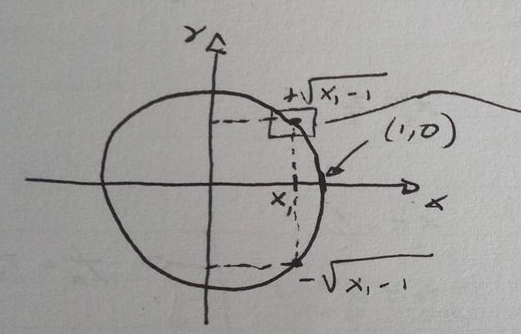
\includegraphics[width=0.5\textwidth]
			{images/f_impl1.png}
			\caption{\label{fig:my-label}}}
	\end{figure}
	
	Se però restringiamo il campo di studio nel seguente modo
	\begin{figure}[!htb]
		\center{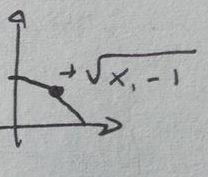
\includegraphics[width=0.3\textwidth]
			{images/f_impl2.png}
			\caption{\label{fig:my-label}}}
	\end{figure}
	
	Notiamo che abbiamo un grafico di funzione validissimo.
\end{enumerate}

Quello che traiamo da questi due esempi è che affinché sia definita una funzione implicta devono esserci condizioni molto stringenti, e sarà valido solo per ben definite regioni di piano. 

\bigskip

Ci viene in aiuto il teorema di Dini, nelle prossime pagine.

\newpage 
\subsection{Th. di Dini per funzioni scalari ad una variabile}

\textit{siano $\deffuncR{2}{}$ tale che}
\begin{enumerate}
	\item $f\in C^0(A)$
	\item $\exists f_y\in C^0(A)$
\end{enumerate}

\textit{e $(x_0,y_0)\in A$ tale che}

\begin{enumerate}
	\item $f(x_0,y_0)=0$
	\item $f_y(x_0,y_0)\neq0$
\end{enumerate}

\textit{Allora si ha che}
\begin{align}
	{}&\exists I(x_0),J(y_0) \taleche I \times J \in A\\ 
	&I \times J\taleche \exists ! y \in J \taleche f(x,y)=0
\end{align}

\textit{Possiamo quindi definire l'applicazione}
\begin{align}
	g=g(x) \taleche I \longrightarrow J \spacer g(x)\in C^0(I)
\end{align}

\textit{definita implicitamente da $f(x,g(x))=0$, con l'unicità di $y$ che impone $g(x_0)=y_0$.}

\bigskip

Il teorema può essere dimostrato in diversi modi. Quello che noi useremo si appoggia al \textbf{principio delle contrazioni}. La dimostrazione si snoda in tre passi, che vediamo dalla pagina successiva.

Come step preliminare riscriviamo la tesi in modo comodo
\begin{align}
	{}&f(x,y)=0 \leftrightarrow \frac{f(x,y)}{f_y(x_0,y_0)}=0 \leftrightarrow y-\frac{f(x,y)}{f_y(x_0,y_0)}=y\leftrightarrow G(x,y)=y\\
	&G(x_0,y_0)= y_0-\frac{f(x_0,y_0)}{f_y(x_0,y_0)}=y_0 - 0 = y_0\\
	&G_y(x,y)= 1- \frac{f_y(x,y)}{f_y(x_0,y_0)} \\
	&G_y(x_0,y_0)= 1 - \frac{f_y(x_0,y_0)}{f_y(x_0,y_0)} = 1 - 1=0
\end{align}

E definendo gli intorni come
\begin{align}
	{}&I(x_0)= (x_0 - r \spacecomma x_0 + r)\\
	&J(y_0)= (y_0 - \epsilon \spacecomma x_0 + \epsilon)\\
	&\overline{I} \times \overline{J}\in A
\end{align}

\begin{enumerate}
	\item \textbf{I passo:} Dimostrare che $(X,||\cdot||_\infty)$ è uno spazio metrico completo, dato $X= \{g\in C^0(I) \taleche ||g-y_=||_\infty <\epsilon\}$
	
	Ci basta trovare una successione di Cauchy $g_n$ tale che 
	\begin{align}
		\{g_n\} \in X \taleche g_n \longrightarrow \vecx \in X \subset C^0(\overline{I})
	\end{align}
	Siccome già sappiamo che 
	\begin{align}
		{}&\{g_n\} \text{ di Cauchy in } C^0(\overline{I}) \text{ completo}\\	
		&\exists g \in C^0(\overline{I}) \taleche g_n
		\overset{||\cdot||_\infty}{\longrightarrow} g
	\end{align}
	Ci basta dimostrare che $g\in X$. Siccome $g_n \in  X$ allora
	\begin{align}
		| g_n(x) - y_0| < || g_n(x) - y_0||_\infty \leq \epsilon \quad \forall x \in \overline{I}
	\end{align}
	
	Siccome $g_n \arrowlim{n}{\infty} g$ si ha che 
	\begin{align}
		\limit{n}{\infty}| g_n(x) - y_0| = | g(x) - y_0|\leq \epsilon \quad \forall x \in \overline{I}
	\end{align}
	
	Che implica a sua volta
	\begin{align}
		|| g(x) - y_0||_\infty\leq \epsilon \quad \forall x \in \overline{I} \implies g(x)\in X
	\end{align}
	
	e abbiamo finito il primo passo.
	
	\newpage
	
	\item \textbf{II passo:} Cerchiamo ora di dimostrare come $G(x,g(x))$ sia una contrazione. Ovvero definita
	\begin{align}
		T[g](x) = G(x,g(x)) \taleche X \longrightarrow C^0(\overline{I})
	\end{align}
	Innanzitutto ci serve che
	\begin{enumerate}
		\item $X= C^0(\overline{I})$
		\item $||T[g](x) - y_0||_\infty$
	\end{enumerate}
	Sia ora $x \in I$, avremo che
	\begin{align}
		|T[g] - y_0| {}&= |G(x,g(x)) - y_0| = |G(x,g(x)) - G(x_0,g(x_0))|= \continue
		&= |G(x,g(x)) - G(x_0,g(x_0))  + G(x,y_0) - G(x,y_0)|\leq \continue
		&\leq |G(x,g(x)) - G(x,y_0)| + |G(x,y_0) - G(x_0,g(x_0))|   
	\end{align}
	Studiamo separatamente i due pezzi:
	\begin{enumerate}
		\item Facendo uso di Lagrange 1D, e ponendoci in 
		\begin{align}
			\eta \in [y_0 \spacecomma g(x)]\subset [y_0 - \epsilon \spacecomma y_0 + \epsilon ]
		\end{align}
		Potremo scrivere
		\begin{align}
			|G(x,g(x)) - G(x,y_0)| {}&= |G(x,\eta) (g(x) - y_0)| \leq  \continue 
			&\leq \half |g(x) - y_0|  \leq \continue
			&\leq \half ||g(x) - y_0||_\infty \leq \half \epsilon
		\end{align}
		Questo perché, essendo $G_y(x_0,y_0)=0$, in un intorno di tale punto si ha che $G_y(x,y)$ è molto piccola e si può maggiorare con $\half$.
		
		\item Il secondo pezzo è più semplice, basta proseguire nel seguente modo:
		\begin{align}
			{}&|G(x,y_0) - G(x_0,g(x_0))| \leq \half \epsilon \quad \forall x \in I(x_0)\\ 
			&I(x_0)\subset [x_0 - r \spacecomma x_0 + r]
		\end{align}
	\end{enumerate}
	Da cui segue infine 
	\begin{align}
		|T[g] - y_0| \leq \half \epsilon + \half \epsilon = \epsilon \implies \underset{I}{max}|T[g] - y_0| \leq \epsilon \quad \forall x \in \overline{I}
	\end{align}
	Il che vuol dire che
	\begin{align}
		||T[g] - y_0||_\infty \leq  \epsilon \quad \forall x \in \overline{I}
	\end{align}
	Che è il risultato cercato.
	
	\item \textbf{III passo:} Dimostriamo l'altra condizione affinché $G(x,g(x))$ sia una contrazione, ovvero che
	\begin{align}
		\exists \alpha \in (0,1) \taleche ||T[g] - T[h]||_\infty \leq \alpha || g -h  ||_\infty 
	\end{align}
	Avremo che
	\begin{align}
		||T[g] - T[h]||_\infty = ||G(x,g(x)) - G(x,h(x))||_\infty
	\end{align}
	Usando di nuovo il th. di Lagrange nello stesso modo del punto precedente avremo
	\begin{align}
		||T[g] - T[h]||_\infty = ||G_y(x,\eta) (g(x) -h(x))||_\infty
	\end{align}
	Analogamente a prima, dato che  $G(x_0,y_0)=0= G_y(x_0,y_0)$ avremo che per $\forall \eta \in [h(x)\spacecomma g(x)]\subset[y_0 - \epsilon \spacecomma y_0 + \epsilon]$
	Sicuramente avremo
	\begin{align}
		|G_y(x,\eta)|\leq \half
	\end{align}
	Ma essendo $\half \in (0,1)$ lo possiamo assumere come valore di $\alpha$! Ci troviamo quindi ad avere
	\begin{align}
		||G(x,g(x)) - G(x,h(x))||_\infty = \half||g(x) - h(x)||_\infty
	\end{align}
	E abbiamo così dimostrato come $G(x,g(x))$ sia una contrazione! Possiamo quindi chiudere la dimostrazione applicando il \textbf{Principio di contrazione}:
	\begin{align}
		\exists ! g \in X \taleche T[g](x)) = g(x)\\
		\updownarrow \continue 
		G(x,g(x))=g(x) \\
		\updownarrow \continue
		f(x,g(x))=0
	\end{align}
\end{enumerate}

\newpage

Il th. di Dini ci garantisce l'esistenza, ma non  ci dice che forma abbia $g(x)$. 

Ci serve quindi di enunciare il seguente \textbf{teorema}:

\bigskip

\textit{Se valgono le ipotesi del teorema di Dini, con aggiunta la condizione}
\begin{align}
	\exists f_x(x,y)\in C^0(A)\implies f(x,y)\in C^1(A)
\end{align}
\textit{Allora possiamo scrivere}
\begin{align}
	g'(x)= - \frac{f_x(x,y)}{f_y(x,y)}
\end{align}
\textit{E se $f\in C^k(I)$ allora avremo che}
\begin{align}
	g^{(k)}(x) = \dertotk{k-1}{}{x} g'(x)= - \dertotk{k-1}{}{x} \left( \frac{f_x(x,y)}{f_y(x,y)} \right)
\end{align}

\bigskip

Per la dimostrazione iniziamo ponendo
\begin{align}
	{}&f(x,g(x))= 0 \implies f(x+h,g(x+h))=0 \quad \forall x \spacecomma x+h \in I(x_0) \nextpassage
	&f(x+h,g(x+h)) - f(x,g(x)) = 0
\end{align}
Il th. di Lagrange in due variabili afferma che
\begin{align}
	f(x_1,y_1) - f(x_2,y_2) = f_x(x_3,y_3)(x_1-x_2) + f_y(x_3,y_3)(y_1 - y_2) 
\end{align}
Da cui otteniamo, posto $(\xi,\eta)\in [(x+h,g(x+h)) \spacecomma (x,g(x))]$
\begin{align}
	{}&0=f(x+h,g(x+h)) - f(x,g(x)) = f_x(\xi,\eta)h+ f_y(\xi,\eta) (g(x+h) - g(x)) \nextpassage
	&f_x(\xi,\eta)h=  - f_y(\xi,\eta) (g(x+h) - g(x)) \nextpassage
	&\frac{g(x+h) - g(x)}{h} = - \frac{f_x(\xi,\eta)}{f_y(\xi,\eta)} \nextpassage
	&\limit{h}{0} \frac{g(x+h) - g(x)}{h} = - \limit{h}{0} \frac{f_x(\xi,\eta)}{f_y(\xi,\eta)}
\end{align}
Siccome per $h\rightarrow 0$ si ha che
\begin{align}
	{}&(\xi,\eta)\in [(x+h,g(x+h)) \spacecomma (x,g(x))] \arrowlim{h}{0} [(x,g(x)) \spacecomma (x,g(x))] \nextpassage
	&(\xi,\eta) = (x,g(x))
\end{align}
Allora si ottiene il risultato cercato
\begin{align}
	{}&g'(x)=\limit{h}{0} \frac{g(x+h) - g(x)}{h} = - \limit{h}{0} \frac{f_x(\xi,\eta)}{f_y(\xi,\eta)} = - \frac{f_x(x,y)}{f_y(x,y)} \nextpassage
	&g'(x)= - \frac{f_x(x,y)}{f_y(x,y)}
\end{align}

Una dimostrazione più semplice ma che può essere applicata solo per funzioni di classe $C^1$ si basa sulla formula delle derivate di funzioni composte che già conosciamo.

\bigskip

\textbf{Nota bene:} Tutti i risultati ricavati finora possono essere ricavati a variabili invertite, basta scambiare le condizioni.

\bigskip

Chiudiamo il discorso mostrando l'espresione delle derivate al II ordine:
\begin{align}
	{}&f \in C^2(A) \implies g\in C^2(A)\\
	&g'(x) = - \frac{f_x(x,y)}{f_y(x,y)} \nextpassage
	&g'(x)f_y(x,y) = -f_x(x,y) \nextpassage
	& g'(x)f_y(x,y) + f_x(x,y)=0 \nextpassage
	&\dertot{}{x} (g'(x)f_y(x,y) + f_x(x,y))=0 \nextpassage
	&f_{xx}(x,y) + f_{xy}(x,y)g'(x) + [f_{xy}(x,y) + f_{yy}(x,y)g'(x)]\cdot g'(x) + f_y(x,y)g''(x)=0 \nextpassage
	& f_{xx}(x,y) + 2f_{xy}(x,y)g'(x) + f_{yy}(x,y)[g'(x)]^2 + f_y(x,y)g''(x)=0\nextpassage
	&g''(x) = -\frac{f_{xx}(x,y) + 2f_{xy}(x,y)g'(x) + f_{yy}(x,y)[g'(x)]^2}{f_y(x,y)}
\end{align}

Se $g'(x)=0$ l'espressione si semplifica notevolmente in $g''(x) = -\frac{f_{xx}(x,y)}{f_y(x,y)}$

\subsection{Esempi di esercizi}

\begin{enumerate}
	\item Data l'equazione
	\begin{align}
		x \Exp{y}=y
	\end{align}
	
	\begin{enumerate}
		\item Dire se in un intorno di $(0,0)$ essa descrive una curva $(x,g(x))$
		\item Determinare l'equazione della retta tangente alla curva in $x=0$
		\item Tracciare un grafico approssimativo
	\end{enumerate}
	
	\bigskip
	Procediamo in ordine:
	\bigskip
	
	\begin{enumerate}
		\item Verifichiamo se la nostra $f(x,y)= x \Exp{y}-y$ rispetta le condizioni di Dini:
		\begin{align}
			{}& f \in C^k(\R^2) \quad \forall k\\ 
			&f(0,0)= 0\\
			&f_y(x,y)= x \Exp{y}-1 \implies f_y(0,0)= 0-1 = -1 \neq 0 \\
			&f_x(x,y)= \Exp{y} \implies f_x(0,0)= 1
		\end{align}
		Le condizioni sono rispettate, quindi avremo
		\begin{align}
			{}&\exists I(x_0)\times J(y_0) \subset A \taleche \forall x\in I(x_0) \quad \exists ! y \in J(y_0) \taleche x\Exp{y}-y=0\\
			& y = y(x) \taleche I \longrightarrow J \spacer g(0)=0 \spacer g^k(I)
		\end{align}
		
		\item La retta tangente è data da\begin{align}
			{}&y= y_0 + g'(x_0)(x-x_0)= 0 - \left. \frac{f_x}{f_y}\right|_{(0,0)}x= 0 - \frac{1}{-1}x=x\nextpassage
			&y -x =0
		\end{align} 
		
		\item Per tracciare il grafico della funzione abbiamo bisogno delle derivate successive
		\begin{align}
			{}&f_{xx} = 0 \implies f_{xx}(0,0) = 0\\
			&f_{xy} = \Exp{y}=f_{yx} \implies f_{xy}(0,0) = 1\\
			&f_{yy}= x\Exp{y}\implies f_{yy}(0,0) = 0\\
			&g''(0)= -\frac{0 +2 + 0}{-1}=2
		\end{align}
		
		E con Taylor avremo
		\begin{align}
			g(x)= g(0) + g'(0)x + \half g''(0)x^2 + o(x^2)= 0+x+x^2 + o(x^2)
		\end{align}	
	\end{enumerate}
		
	\item Data l'equazione
	\begin{align}
		e^x \sin(y) + e^y\cos(x)-1=0
	\end{align}
	In un intorno di $(0,0)$
	\begin{enumerate}
		\item Verificare l'esistenza di una funzione implicita 
		\item Verificare che in $x=0$ abbia un punto critico
		\item Categorizzare tale punto
	\end{enumerate}
	
	\bigskip
	\begin{enumerate}
		\item Verifichiamo le condizioni di Dini
		\begin{align}
			{}&f\in C^k(I)\\
			& f(0,0)=1-1=0\\
			& f_y= e^x \cos(y) + e^y\cos(x) \implies f_y(0,0)= 1+1=2\neq 0 \\
			& f_x= e^x \sin(y) - e^y\sin(x) \implies f_y(0,0)= 1\cdot 0+0\cdot 1= 0
		\end{align}
		
		Le condizioni sono verificate, e abbiamo quindi sicuro una $g(x)$
		
		\item Verificare che in $x=0$ abbia un punto critico
		\begin{align}
			g'(0)=-\frac{f_x(0,0)}{f_y(0,0)}=-\frac{0}{2}=0
		\end{align}
		Quindi $x=0$ è punto critico
		
		\item Categorizziamo tale punto
		\begin{align}
			f_{xx}= e^x \sin(y) - e^y\cos(x) \implies f_{xx}(0,0)= -1
		\end{align}
		Siccome $g'(0)=0$ possiamo usare la forma ridotta
		\begin{align}
			g''(0)= -\frac{f_{xx}(0,0)}{f_y(0,0)}= - \frac{-1}{2}= \half > 0 
		\end{align}
		E quindi $x=0$ è un punto di minimo. 
	\end{enumerate}
	
	\item Data l'equazione
	\begin{align}
		y^2 + x+ \Exp{x^2 + y^2} -1 =0
	\end{align}
	
	Studiamo le stesse richieste del precedente esercizio in un intorno di $(0,0)$, con aggiunto il calcolo della retta tangente.
	
	\begin{enumerate}
		\item Verifichiamo le condizioni di Dini
		\begin{align}
			{}&f\in C^k(I)\\
			& f(0,0)=0+0+ 1-1=0\\
			& f_y= 2y(1+\Exp{x^2 + y^2})\implies f_y(0,0)= 0 \\
			& f_x= 1 + 2\Exp{x^2 + y^2} \implies f_x(0,0)= 1+0=1\neq 0
		\end{align}
		Ci troviamo stavolta nel caso opposto, che avevamo brevemente detto esistere. Avremo cioè che
		\begin{align}
			\exists I(x_0)\times J(y_0) \taleche \forall y \in J \quad \exists ! x \taleche f(h(y),y)=0
		\end{align} 
		
		\item Avremo in $y=0$ un punto critico, infatti
		\begin{align}
			h'(0)= -\frac{f_y(0,0)}{f_x(0,0)} =0
		\end{align}
		
		\item Per classificare $y=0$ ci basta calcolare
		\begin{align}
			{}&f_{yy}(0,0)= [2(1+\Exp{x^2 + y^2}) - 4y^2\Exp{x^2 + y^2}]|_{(0,0)}= 4\\&h''(0)=-\frac{f_{yy}(0,0)}{f_x(0,0)}=-4
		\end{align}
		Abbiamo quindi un punto di massimo
		
		\item La retta tangente avrà equazione
		\begin{align}
			h(y)= h(0) + h'(0)y + \half h''(0)y^2 + o(y^2)= 2y^2 + o(y^2)
		\end{align}
	\end{enumerate}
\end{enumerate}

\newpage

\subsection{Teorema di Dini per funzioni scalari a più variabili}
\textit{Siano}
\begin{align}
	{}&\vecx= (x_1,\dots, x_n)\in \R^n\spacer y \in \R\\
	&f(\vecx,y) \taleche A \subseteq \R^{n+1} \longrightarrow \R
\end{align}
\textit{Se valgono le seguenti condizioni in $(\vecx^0,y_0)\in A$}
\begin{enumerate}
	\item $f(\vecx,y)\spacecomma f_y(\vecx,y)\in C^0(A)$
	\item $(\vecx^0,y_0) \taleche f(\vecx^0,y_0) =0 \neq f_y(\vecx^0,y_0)$ 
\end{enumerate}
\textit{Allora si ha che}
\begin{align}
	{}&\exists I(\vecx^0) = \{\vecx \taleche |\vecx - \vecx^0|\leq r \} \text{ intorno sferico}\\
	&\exists J(y_0)=(y_0-\epsilon \spacecomma y_0+\epsilon)
\end{align}
\textit{con}
\begin{align}
	I \times J \subset A \taleche \forall \vecx \in I \quad \exists ! y \taleche f(x,y)=0 \leftrightarrow y= g(\vecx) \taleche I\longrightarrow J
\end{align}
\textit{Inoltre se $f\in C^1(A)$ si ha che anche $g\in C^1(I)$ e si può scrivere}
\begin{align}
	g_{x_i}= - \frac{f_{x_i} (\vecx,g(\vecx))}{f_y(\vecx,g(\vecx))}
\end{align}

\bigskip
Non diamo la dimostrazione del teorema, non essendoci necessaria ai fini del corso. Ci chiediamo però: in termini pratici, che ci dice questa versione del teorema? Notiamo come in realtà sia una forma più generale del caso che abbiamo già enunciato, che è qui rappresentato nel caso $n=1$, mentre il caso $n=2$ sarà
\begin{align}
	{}&\deffuncR{3}{}\\
	&\Sigma = \{\vecP = (x,y,z) \taleche f(\vecP)=0 \}\\
	& \vecP^0\in A \taleche f(\vecP^0)=0\neq f_z(\vecP^0)\\
	&z= g(x,y) \\
	&g_x = - \left. \frac{f_x}{f_z}\right|_{\vecP^0} \spacer g_y = - \left. \frac{f_y}{f_z}\right|_{\vecP^0}\\
	&T(z,\vecP^0)= z_0 + g_x(x_0,y_0) (x-x_0) + g_y(x_0,y_0)(y-y_0)
\end{align}

Vediamo, per chiarirci di più le idee, un \textbf{esempio:}
\begin{align}
	{}&\Exp{z} + z\Exp{x+y} - \Exp{x-y}=0 \implies f(x,y,z)= \Exp{z} + z\Exp{x+y} - \Exp{x-y}\\
	& f\in C^k(\R^3) \quad \forall k\\
	& f_z(x,y,z)= \Exp{z} + \Exp{x+y} \implies f_z(0,0,0)= 1+1 = 2 \neq 0
\end{align}

Avremo quindi
\begin{align}
	g(x,y)	\in C^k(I) \quad \forall k \taleche I(0,0) \subset \R^2 \longrightarrow J(0,0) \subset \R 
\end{align}

Andiamo a calcolarne il piano tangente:
\begin{align}
	{}&f_x= z\Exp{x+y} - \Exp{x-y} \implies f_x(0,0) = -1 \\
	&f_y = z\Exp{x+y} + \Exp{x-y}\implies f_y(0,0) = +1 \\
	&T(z,\vecP^0) = 0 - \left(\half\right)x - \left(\half\right)y= \half (x-y)
\end{align}

\newpage 

\subsection{Teorema di Dini per sistemi di funzioni}

Poniamoci ora la seguente domanda: chi chiediamo se il sistema
\begin{align}
	\double{f(x,y,z)=0}{g(x,y,z)=0}
\end{align}
Possa definire una curva $\gamma$ tale che
\begin{align}
	\underline{r}(t)=\triple{x=t}{y=y(t)}{z=z(t)}
\end{align}

La risposta è: dipende.

Ad esempio col seguente sistema
\begin{align}
	\double{ax + by + cz + d=0}{\alpha x + \beta y + \gamma z  + \delta=0} \implies \double{ by + cz =- d -ax}{\beta y + \gamma z =  - \delta - \alpha x}
\end{align}

Avremo una soluzione solo se è rispettata la \textbf{condizione di Kramer}, ovvero
\begin{align}
	\det \matrixTwoTwo{b}{c}{\beta}{\gamma} \neq 0
\end{align}

Affinché quindi abbia soluzione il sistema e si possa definire la curva che rappresenta l'intersezione tra i due piani servono condizioni restrittve. 

Enunciamo il \textbf{Teorema di Dini per sistemi di funzioni:}

\bigskip

\textit{Se si ha}
\begin{align}
	{}&f(x,y,z),g(x,y,z) \in C^1(A) \spacecomma A\subset \R^3\\
	&\vecP^0=(x_0,y_0z_0) \taleche f(\vecP^0)=0=g(\vecP^0) \spacer \det \left. \matrixTwoTwo{f_y}{f_z}{g_y}{g_z}\right|_{\vecP^0}\neq 0
\end{align}
\textit{Allora avremo che}
\begin{align}
	{}&\exists I(x_0) = (x_0 - r \spacecomma x_0 +r) \spacecomma J(x_0,y_0)\subset \R^2\\
	&I \times J \subset A \taleche \exists ! (y,z)\in J \text{ soluzioni del sistema } \double{f(x,y,z)=0}{g(x,y,z)=0} \taleche \double{y=y(x)}{z=z(x)} \text{ per } x\in I
\end{align}

Che forma avranno le derivate? Proviamo a calcolarle
\begin{align}
	{}&\double{f(x,y,z)=0}{g(x,y,z)=0} \implies \double{f_x + f_y y' + f_z z'=0}{g_x + g_y y' + g_z z'=0} \nextpassage 
	&\double{f_x +  f_z z' = -f_y y' }{g_x + g_z z'=-g_y y'} \spacer \double{f_y y' +  f_z z'= -f_x }{g_y y'+ g_z z'=-g_x}
\end{align}

Come nell'esempio prima avremo che devono valere
\begin{align}
	\det \matrixTwoTwo{-f_x}{f_z}{-g_x}{g_z} \neq 0 \spacer \det \matrixTwoTwo{f_y}{-f_x}{g_y}{-g_x} \neq 0
\end{align}
Da cui ricaviamo
\begin{align}
	y'(x)= - \left. \frac{\matrixTwoTwo{-f_x}{f_z}{-g_x}{g_z}}{\det  \matrixTwoTwo{f_y}{f_z}{g_y}{g_z}} \right|_{(x,y)}
	\spacer
	z'(x)= - \left. \frac{\matrixTwoTwo{f_y}{-f_x}{g_y}{-g_x}}{\det  \matrixTwoTwo{f_y}{f_z}{g_y}{g_z}} \right|_{(x,y)}
\end{align}

\newpage 

\subsection{Teorema di Dini nel caso generale}

\textit{Siano}
\begin{align}
	\vecf \taleche A \R^{n+m} {}&\longrightarrow \R^m\\
	(\vecx,\vecy) &\longrightarrow \vecf(\vecx,\vecy)= (f_1,\dots,f_m)|_{(\vecx,\vecy)} \continue
	\vecx=(x_1,\dots,x_n) &\spacer \vecy=(y_1,\dots , y_m)
\end{align}
\textit{Se dato $(\vecx^0,\vecy^0)$ sono rispettate le seguenti proprietà}
\begin{align}
	{}&\vecf \in C^1(A)\\
	&(\vecx^0,\vecy^0) \taleche 	\vecf(\vecx^0,\vecy^0)=0\\
	&\det \left.\left(\partialder{\vecf}{\vecy}\right)\right|_{\vecP^0} \neq 0 \spacer \left(\partialder{\vecf}{\vecy}\right) = \left(\partialder{f_i}{y_j}\right)_{\scriptsize{\begin{array}{cc}
				i=1,\dots,m\\
				j=1,\dots,n
	\end{array}}}
\end{align}
\textit{Allora si ha che esistono}
\begin{align}
	\exists I(\vecx^0) \subset \R^n \spacecomma J(\vecy^0)\subset \R^m \taleche I\times J \subset \R^{n+m}
\end{align}
\textit{Tali che}
\begin{align}
	{}&\forall \vecx\in I \quad\exists ! \vecy \taleche \vecf(\vecx,\vecy) =\veczero\\
	&\vecy = \vecg(\vecx)\in C^1(I)\taleche I\subset \R^n \longrightarrow J \subset \R^m \\
	&\jacobian \vecg(\vecx)= -  \left(\partialder{\vecf}{\vecy}\right)^{-1} \left(\partialder{\vecf}{\vecx}\right)
\end{align}

\subsection{Invertibilità Locale}

Un'interessante applicazione del teorema di Dini si ha nello studio dell'invertibilità locale delle funzioni.

Supponiamo di avere
\begin{align}
	\vecf \taleche A \subset \R^n \longrightarrow B \subset \R^n
\end{align}
Con $A,B$ aperti e $\vecf(\vecx)\in C^1(A)$.

Ci chiediamo: sotto quali ipotesi $\vecf$ è invertibile localmente in $A$, con $\vecf^{-1}\in C^1(B)$? O, in altri termini, quando $\vecf$ è un \textbf{diffeomorfismo} locale tra $A$ e $B$? 

Ci viene in aiuto il \textbf{Teorema di Inversione Locale:}

\bigskip

\textit{Siano}
\begin{align}
	{}&\vecf \taleche A \subset \R^n \longrightarrow B \subset \R^n\\
	&f\in C^1(A)\\
	&\vecx^0 \in A
\end{align}
\textit{Se}
\begin{align}
	\det \jacobian{\vecf}{\vecx^0} = \det\left( \partialder{f_i}{x_j} \right)_{\scriptsize{
			\begin{array}{cc}
				i=1,\dots,n\\
				j=1,\dots n
			\end{array}
	}} \neq 0
\end{align}
\textit{Allora f è localmente invertibile.}

\bigskip

La dimostrazione discende dal caso generale di Dini. 

Posti
\begin{align}
	{}&\vecF (\vecx,\vecy)= \vecy - \vecf(\vecx)\\
	& \vecy^0 = \vecf(\vecx^0)
\end{align}
Applichiamo Dini in $(\vecx^0,\vecy^0)$. Le ipotesi sono verificate per costruzione, dato che
\begin{align}
	{}&\vecF (\vecx^0,\vecy^0)= \vecy^0 - \vecf(\vecx^0) = \vecy^0 - \vecy^0 =0\\
	&\vecF\in C^1(A \times \R^n)\\
	& \left. \partialder{\vecF}{\vecx} \right|_{(\vecx^0,\vecy^0)} = - \left. \partialder{\vecf}{\vecx} \right|_{(\vecx^0,\vecy^0)} \neq 0 \text{ per ipotesi}
\end{align}
Questo vuol dire che
\begin{align}
	\exists I(\vecx^0),J(\vecy^0) \taleche \forall \vecy \in J \quad \exists \vecx = \vech(\vecy) \in I \taleche \vecF (\vech(\vecy),\vecy) =0
\end{align}
Ma questo vuol dire anche che
\begin{align}
	\vecy = \vecf(\vech(\vecy)) \implies \vech(\vecy)= \vecf^{-1}(\vecy)
\end{align}
E il teorema è dimostrato.

\bigskip

Le derivate avranno forma
\begin{align}
	\partialder{\vech(\vecy)}{\vecy} = -\left( \partialder{\vecF}{\vecx} \right)^{-1}\left( \partialder{\vecF}{\vecy} \right)
\end{align}
Ma per come abbiamo definito $\vecF$ il secondo termine diventa
\begin{align}
	\partialder{\vech(\vecy)}{\vecy} = -\left( \partialder{\vecF}{\vecx} \right)^{-1} \mathbb{1}_n = -\left( \partialder{\vecF}{\vecx} \right)^{-1} \implies \jacobian{f^{-1}}{\vecx}= (\jacobian{f}{\vecx})^-1
\end{align}
Ma a noi tutto questo è familiare! Infatti in $\R$ avevamo che se
\begin{align}
	y=f(x)\in C^1((a,b)) \spacer f'(x_0)\neq 0 \spacecomma x_0\in (a,b)
\end{align}
Allora 
\begin{align}
	\dertot{}{y}f^{-1}(y)= \fracn{f'(f^{-1}(y))}
\end{align}
La differenza giace però nell'invertibilità globale. Infatti mentre in $\R$ la derivabilità in tutto l'insieme implica monotonia e quindi invertibilità in tutto l'insieme, in $\R^{n>1}$ non è detto, come vediamo nel seguente \textbf{esempio in $\R^2$:}
\begin{align}
	{}&\vecy = \vecf(\vecx)= \double{y_1= \Exp{x_1} \cos(x_2)}{y_2= \Exp{x_1} \sin(x_2)}\\
	\continue
	& \jacobian{\vecf}{\vecx}=\partialder{\vecf}{\vecx}= \matrixTwoTwo{f_{1_{x_1}}}{f_{1_{x_2}}}{f_{2_{x_1}}}{f_{2_{x_2}}} = \matrixTwoTwo{+\Exp{x_1} \cos(x_2)}{-\Exp{x_1} \sin(x_2)}{+\Exp{x_1} \sin(x_2)}{+\Exp{x_1} \cos(x_2)}
\end{align}
Da cui segue che 
\begin{align}
	\det \jacobian{\vecf}{\vecx}= \Exp{2x}\neq 0 \quad \forall \vecx
\end{align}
Però la funzione non è iniettiva, e quindi non può essere invertibile globalmente. 

\section{Punti di massimo e minimo vincolati}

Per amor di semplicità studiamo il problema nel piano.

Dati
\begin{align}
	{}&\deffuncR{2}{}\\
	&\deffuncRgen{g}{2}{}\\
	&Z= \{ (x,y)\in A \taleche g(x,y)=0 \}\neq \emptyset
\end{align}
Definiamo $(x_0,y_0)$ 
\begin{enumerate}
	\item \textbf{punto di max. vincolato di $f$ su Z} se
	\begin{align}
		f(x,y)\leq f(x_0,y_0) \quad \forall (x,y)\in Z \cap I(x_0,y_0)
	\end{align}
	\item \textbf{punto di min. vincolato di $f$ su Z} se
	\begin{align}
		f(x,y)\geq f(x_0,y_0) \quad \forall (x,y)\in Z \cap I(x_0,y_0)
	\end{align}
\end{enumerate}

Ci domandiamo: perché stiamo studiando di nuovo il problema? Non abbiamo già il teorema di Fermat? La risposta è \textbf{no}, visto che Fermat considera \underline{solo} gli insiemi aperti!

\bigskip

Siamo quindi costretti a trovare altre vie per tale studio. 

\bigskip

Un metodo lo conosciamo già, dato che $Z$ è una curva: parametrizziamo nel seguente modo
\begin{align}
	Z=\{ (x(t),y(t)) \spacecomma t \in [a,b] \}
\end{align}
E ci troviamo a studiare una funzione in $\R$, dove abbiamo tutti gli strumenti per lavorare:
\begin{align}
	f(x,y)|_Z = f(x(t),y(t)) =F(t)
\end{align}

\bigskip

Un altro metodo molto interessante è quello dei \textbf{Moltiplicatori di Lagrange}, che vediamo nella pagina successiva.

\newpage

\subsection{Metodo dei Moltiplicatori di Lagrange in $\R^2$}

\textit{Se abbiamo}
\begin{enumerate}
	\item $f,g \in C^1(A)$
	\item $(x_0,y_0)\in A$ tale che
	\begin{enumerate}
		\item $g(x_0,y_0)=0 \leftrightarrow (x_0,y_0)\in Z$
		\item $\gradient{g}{x_0,y_0}\neq 0 \leftrightarrow (x_0,y_0)$ punto regolare
		\item $(x_0,y_0)$ punto di max. (o min.) vincolato per $f$
	\end{enumerate}
\end{enumerate}

\textit{Allora avremo un risultato che può essere enunciato in tre modi equivalenti:}
\begin{enumerate}
	\item $\left. \det \matrixTwoTwo{f_x}{f_y}{g_x}{g_y}\right|_{(x_0,y_0)} = 0$
	\item $\exists \lambda_0 \in \R \taleche \gradient{f}{x_0,y_0}= \lambda_0 \gradient{f}{x_0,y_0}$
	\item \textit{Data }$L(x,y,\lambda)= f(x,y) - \lambda g(x,y)$ $\exists \lambda_0 \taleche \gradient{L}{x_0,y_0, \lambda_0}=\veczero$ 
\end{enumerate}

Prima di dare la dimostrazione mostriamo perché le tre formulazioni siano equivalenti:

La prima scrittura implica che i gradienti siano \textbf{linearmente dipendeti} e che quindi $\exists \lambda_0 \taleche \gradient{f}{x_0,y_0}= \lambda_0 \gradient{f}{x_0,y_0}$ che è la seconda scrittura.

La terza implica che
\begin{align}
	\triple{L_x(x_0,y_0, \lambda_0) = {}&[f_x - \lambda_0 g_x]|_{(x_0,y_0, \lambda_0)}=0}{L_y(x_0,y_0, \lambda_0) = &[f_y - \lambda_0 g_y]|_{(x_0,y_0, \lambda_0)}=0}{L_\lambda(x_0,y_0, \lambda_0) = &-g|_{(x_0,y_0, \lambda_0)}=0}
\end{align}
La terza derivata è un'ipotesi, le altre due altro non sono che il secondo enunciato.

Vediamo come dimostrare il teorema.

Per ipotesi in $(x_0,y_0)$ abbiamo che
\begin{align}
	g_y(x_0,y_0) \neq 0 = g(x_0,y_0)
\end{align}
Possiamo quindi applicare il teorema di Dini, da cui abbiamo che
\begin{align}
	\exists I(x_0)\times J(y_0) \taleche \forall x \quad \exists ! y=h(x) \taleche f(x,h(x))=0
\end{align}
Sia ora $\vecP^0=(x_0,y_0)$ punto di max.vincolato, ovvero
\begin{align}
	{}&f(x,y)\leq f(x_0,y_0) \quad \forall (x,y)\in Z\cap  I(x_0)\times J(y_0) \nextpassage
	& f(x,h(x)) \leq f(x_0,h(x_0)) \quad \forall x\in I(x_0) \nextpassage
	& F(x)\leq F(x_0)  \quad \forall x\in I(x_0)= (x_0 - r \spacecomma x_0 + r)
\end{align}
Per Fermat avremo che
\begin{align}
	{}&F'(x_0)=0 \nextpassage
	&\dertot{}{x}f(x_0,h(x_0))=0\nextpassage						&f_x(x_0,h(x_0)) + f_y(x_0,h(x_0))h'(x_0)=0\nextpassage
	&f_x(x_0,h(x_0)) - f_y(x_0,h(x_0))\frac{g_x(x_0)}{g_y(x_0)}=0  \quad\text{per il th. di Dini} \nextpassage
	& \frac{f_x(x_0,h(x_0))g_y(x_0) - f_y(x_0,h(x_0))g_x(x_0)}{g_y(x_0)}=0 \nextpassage
	&\fracn{g_y(x_0)} \det \left.\matrixTwoTwo{f_x}{f_y}{g_x}{g_y}\right|_{\vecP^0}=0 \nextpassage
	& \left.\det\matrixTwoTwo{f_x}{f_y}{g_x}{g_y}\right|_{\vecP^0}=0
\end{align}
Che è la nostra prima formulazione, e quindi il th. è dimostrato.

\newpage

Vediamo ora un \textbf{esempio:} la massimizzazione dell'area di rettangoli inscritti in un'ellisse.

\bigskip

Sia l'ellisse di equazione
\begin{align}
	\frac{x^2}{a^2} + \frac{y^2}{b^2}=1 \spacer a,b>0
\end{align}

E sia il rettangolo inscritto
\begin{align}
	f(x,y)= xy
\end{align}

Ci chiediamo
\begin{align}
	\underset{g(x,y)=0}{max}f(x,y)=?
\end{align}

Per quanto riguarda $f(x,y)$ sappiamo che
\begin{enumerate}
	\item $f(x,y)$ è continua su tutto $\R^2$
	\item $f(a,0)=f(0,b)=0$ 
\end{enumerate}

Ponendo ora
\begin{align}
	g(x,y)= \frac{x^2}{a^2} + \frac{y^2}{b^2}-1
\end{align}

E tenendo conto del fatto che la lunghezza dei lati del rettangolo deve essere positiva, avremo
\begin{align}
	Z=\{ (x,y) \taleche g(x,y)=0 \spacer x,y \geq 0 \} \subset [-a\spacecomma +a]\times [-b \spacecomma +b]
\end{align}

\begin{figure}[!htb]
	\center{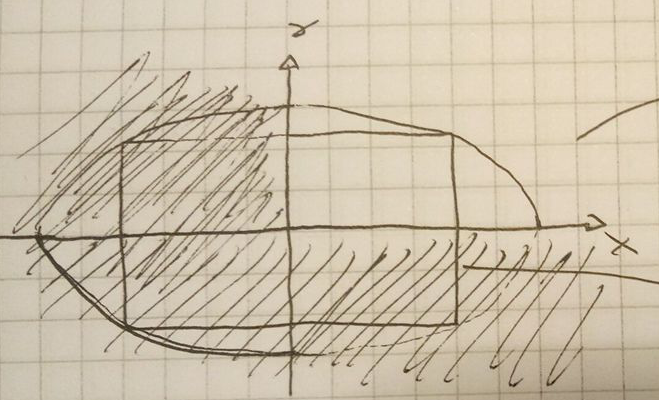
\includegraphics[width=0.5\textwidth]
		{images/esempio.png}
		\caption{\label{fig:my-label}}}
\end{figure}

$Z$ è chiuso e limitato e per Weierstrass sicuro esistono max. e min. su $Z$. 
Il minimo lo sappiamo già ad occhio, visto che abbiamo solo valori non negativi di $x$ e $y$ deve essere che
\begin{align}
	\underset{(x,y)\in Z}{min}f(x,y)=0 \implies (0,b) \spacecomma (a,0) \text{ punti di minimo}
\end{align}
Andiamo a trovare il massimo tramite Lagrange, ma prima accertiamoci che non ci siano punti non regolari:
\begin{align}
	{}&\gradient{g}{x,y}= \veccolTwo{\frac{2x}{a^2}}{\frac{2y}{b^2}} = \veccolTwo{0}{0} \implies (x,y)=(0,0)\\
	&\gradient{f}{x,y}=\veccolTwo{y}{x}=  \veccolTwo{0}{0} \implies (x,y)=(0,0)
\end{align}

Ma l'origine non è compresa in $Z$, quindi nessun problema.

Possiamo quindi applicare Lagrange, costruendo il sistema
\begin{align}
	\double{\det \matrixTwoTwo{y}{x}{\frac{2x}{a^2}}{\frac{2y}{b^2}}=0}{\frac{x^2}{a^2} + \frac{y^2}{b^2}=1}\implies
	\double{\frac{y^2}{b^2} - \frac{x^2}{a^2}=0}{\frac{x^2}{a^2} + \frac{y^2}{b^2}=1}
\end{align}

Da cui si ricava
\begin{align}
	\double{y^2 = \frac{b^2}{a^2}x^2}{\frac{2}{a^2}x^2=1} \implies x = \pm \frac{a}{\sqrt{2}} \spacer y= \pm \frac{b}{\sqrt{2}}
\end{align}

Scartando i risultati negativi per costruzione abbiamo trovato il nostro punto di massimo in
\begin{align}
	(x,y)_M= \left(\frac{a}{\sqrt{2}} \spacecomma \frac{b}{\sqrt{2}}\right)
\end{align}

\subsection{Esempi}

\begin{enumerate}
	\item Massimizzazione dell'area di rettangoli a somma dei lati costante.
	
	\bigskip
	
	Come prima avremo la funzione che descrive il perimetro
	\begin{align}
		f(x,y)=xy \spacer \gradient{f}{x,y}= (y \spacecomma x)
	\end{align}
	Mentre stavolta il vincolo sarà dato dall'equazione
	\begin{align}
		{}&x+y=c>0 \implies g(x,y)= x+y-c\\
		& Z=\{ x,y \geq 0 \taleche x+y=c \}
	\end{align}
	
	\begin{figure}[!htb]
		\center{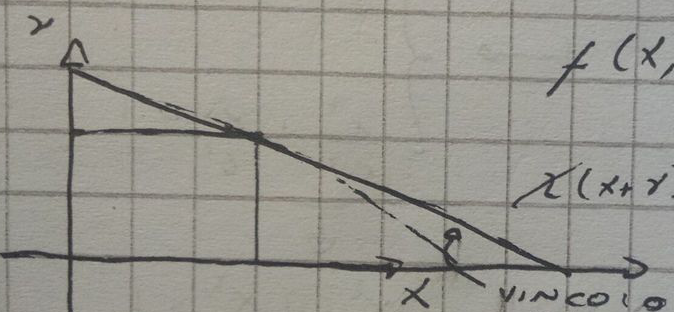
\includegraphics[width=0.5\textwidth]
			{images/esempio2.png}
			\caption{\label{fig:my-label}}}
	\end{figure}	
	
	$Z$ è chiuso e limitato, ergo per Weierstrass ci sono max. e min.
	
	Come nell'esempio precedente il minimo si avrà lungo gli assi, mentre per il massimo utlizziamo Lagrange:
	\begin{align}
		\double{\left.\det\matrixTwoTwo{f_x}{f_y}{g_x}{g_y}\right|_{\vecP^0}=0}{x+y=c} \implies
		\double{x-y=0}{x+y=c}
	\end{align}
	E otteniamo quindi un punto di massimo in
	\begin{align}
		(x,y)_M= \left( \frac{c}{2} \spacecomma \frac{c}{2} \right)
	\end{align}
	
	\bigskip
	
	\item Studiare l'esistenza di punti critici della funzione
	\begin{align}
		{}&f(x,y)= (x+1)^2 + (y-1)^2 \\ 
		&\gradient{f}{x,y} = (2(x+1) \spacecomma 2(y-1))
	\end{align}
	Con vincolo dato da
	\begin{align}
		{}&x^2 + y^2 = 4 \implies g(x,y)=x^2 + y^2 - 4
	\end{align}	
	Nel dominio chiuso e limitato
	\begin{align}
		D = \{ (x,y) \taleche g(x,y)\leq 0 \}
	\end{align}
	
	Siccome
	\begin{align}
		f\in C^0(\R^2) \implies f\in C^0(Z)
	\end{align}
	Quindi per Weierstrass abbiamo punti di massimo e minimo. Dividiamo lo studio in due parti:
	\begin{enumerate}
		\item \underline{punti interni:}
		Non esistono punti di non derivabilità, quindi cerchiamo solo punti critici:
		\begin{align}
			\gradient{f}{x,y} = \veczero \implies \veccolTwo{2(x+1)}{2(y-1)} = \veccolTwo{0}{0}
		\end{align}
		Abbiamo quindi un candidato in
		\begin{align}
			\vecx^0=(-1 \spacecomma +1)
		\end{align}
		
		\item \underline{punti di frontiera:}
		
		La frontiera sarà 
		\begin{align}
			\partial D = \{ x^2 +y^2 =4 \}= \{ (x,y) \taleche g(x,y)=0 \}
		\end{align}
		Assicuriamoci di non avere punti di non regolarità:
		\begin{align}
			\gradient{g}{x,y}= \veccolTwo{2x}{2y} =  \veccolTwo{0}{0} \implies \vecx^?=(0,0)
		\end{align}
		Che non è sulla frontiera, quindi possiamo usare tranquillamente Lagrange.
		\begin{align}
			{}&\triple{  \det \matrixTwoTwo{2(x+1)}{2(y-1)}{2x}{2y} = \det \matrixTwoTwo{x+1}{y-1}{x}{y} =0 }{\quad}{x^2 +y^2 =4} \nextpassage
			& \double{y(x+1) - x(y-1)=0}{x^2 +y^2 =4} \implies \double{y=-x}{2x^2=4} \nextpassage 
			&\double{y=\mp \sqrt{2}}{x=\pm\sqrt{2}} \implies \begin{array}{cc}
				\vecx^1 = (+ \sqrt{2} \spacecomma -\sqrt{2})\\
				\vecx^2 = (- \sqrt{2} \spacecomma +\sqrt{2})
			\end{array}
		\end{align}
		Per vedere quale punto è quale semplicemente calcoliamo la funzione:
		\begin{align}
			{}&f(\vecx^0)=0\\
			&f(\vecx^1)= 2 (\sqrt{2} + 1)^2\\
			&f(\vecx^2)=2 (\sqrt{2} - 1)^2
		\end{align}
		E quindi $\vecx^0$ è chiaramente un punto di minimo e $\vecx^1$ di massimo.
	\end{enumerate}
\end{enumerate}

\newpage

\subsection{Metodo dei Moltiplicatori di Lagrange in $\R^3$}

\textit{Siano}
\begin{enumerate}
	\item $\deffuncRgen{f,g}{3}{} \spacer f,g\in C^1(A)$
	\item $Z= \{ (x,y,z) \taleche g(x,y,z)=0 \}$
	\item $\vecP^0=(x_0,y_0,z_0) \taleche \gradient{g}{\vecP^0}\neq 0 = g(\vecP^0)$
	\item $\vecP^0$ \textit{punto di min./max. vincolato per $f$}
\end{enumerate}
\textit{Allora come nel caso in $\R^2$ abbiamo tre risultati equivalenti:}
\begin{enumerate}
	\item $\partialder{(f,g)}{(x,y,z)}= \matrixThreeTwo{f_x}{f_y}{f_z}{g_x}{g_y}{g_z}$ \textit{ di rango $1$}
	\item $\exists \lambda_0 \taleche \gradient{f}{\vecP^0}=\lambda_0 \gradient{f}{\vecP^0}$
	\item $\mathcal{L}(x,y,z,\lambda)= f(x,y,z) - \lambda_0 \, g(x,y,z) \implies \exists \lambda_0 \taleche \gradient{\mathcal{L}}{\vecP^0,\lambda_0}=0$
\end{enumerate}

\bigskip

Come prima, dimostriamo la prima versione, che implica le altre:

\bigskip

Siccome nelle ipotesi sono verificate le ipotesi di Dini del secondo caso, avremo che
\begin{align}
	\exists I(x_0,y_0)\times J(z_0) \taleche \forall (x,y)\in I(x_0,y_0) \quad \exists ! z= h(x,y) \taleche f(x,y,h(x,y))=0
\end{align}
Sia inoltre $\vecP^0$ punto di maxssimo. Avremo che
\begin{align}
	{}&f(x,y,z)\leq f(\vecP^0) \quad \forall (x,y,z) \in Z \cap I(x_0,y_0) \nextpassage
	&f(x,y,h(x,y))\leq f(x_0,y_0, h(x_0,y_0)) \quad \forall (x,y) \in I(x_0,y_0) \nextpassage
	&F(x,y)= F(x_0,y_0) \quad \forall (x,y) \in I(x_0,y_0)
\end{align}
Ricordando anche i risultati del th. di Dini, per Fermat avremo che
\begin{align}
	{}&F'(x_0,y_0)=0 \nextpassage
	&\dertot{}{x} F(x_0,y_0)=0 \nextpassage
	& \dertot{}{x} f(x_0,y_0, h(x_0,y_0)) = 0 \nextpassage
	& f_x(\vecP^0) + f_z(\vecP^0) h_x(x_0,y_0)=0 \nextpassage
	& \frac{ f_x(\vecP^0)g_z(\vecP^0) - f_z(\vecP^0)g_x(\vecP^0)}{g_z(\vecP^0)}=0\nextpassage
	& f_x(\vecP^0)g_z(\vecP^0) - f_z(\vecP^0)g_x(\vecP^0)=0 \nextpassage
	&\left. \det \matrixTwoTwo{f_x}{f_z}{g_x}{g_z}\right|_{\vecP^0}=0 
\end{align}
Ciò ci dice che la matrice
\begin{align}
	\matrixThreeTwo{f_x}{f_y}{f_z}{g_x}{g_y}{g_z}
\end{align}
è di rango $1$. Il teorema è quindi dimostrato.

\newpage

Vediamo ora un paio di \textbf{esempi:} 

\begin{enumerate}
	\item la massimizzazione del prodotto tra tre variabili non negative a somma costante.
	\begin{align}
		{}&x,y,z\geq 0\\
		&f(x,y,z)=xyz \\
		&x+y+z=c>0 \implies g(x,y,z)=x+y+z-c\\
		&Z=\{ x,y,z \geq 0 \taleche g(x,y,z)=0 \}
	\end{align}
	
	Il problema è equivalente alla massimizzazione del volume di un tetragramma, come si vede in figura
	
	\begin{figure}[!htb]
		\center{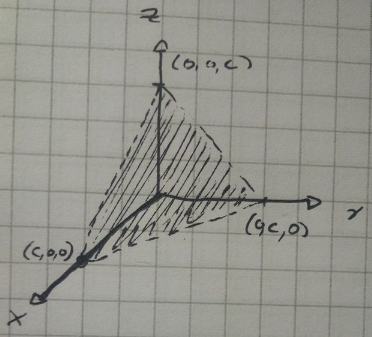
\includegraphics[width=0.5\textwidth]
			{images/esempio3.png}
			\caption{\label{fig:my-label}}}
	\end{figure}	
	
	Calcoliamo i gradienti
	\begin{align}
		{}&\gradient{g}{x,y,z}= (1 \spacecomma 1 \spacecomma 1) \\
		&\gradient{f}{x,y,z}=(yz \spacecomma xz \spacecomma xy)
	\end{align}
	
	Vediamo subito come $g$ non abbia punti di non regolarità, e possiamo quindi applicare Lagrange, dove la prima formulazione della tesi ci porta a scrivere il sistema
	\begin{align}
		\quadruple{yz-xz=0}{xz-xy=0}{yz-xy=0}{x+y+z=c} \implies \quadruple{yz=xz}{xz=xy}{yz=xy}{x+y+z=c}
	\end{align}
	
	Notiamo come la situazione sia un po' intricata.
	
	Se $z=0$ abbiamo che anche $xy=0$ da cui segue che uno dei due deve essere nullo e quindi in automatico anche il rimanente. Ma a noi interessa il massimo, quindi escludiamo valori nulli. Allora avremo
	\begin{align}
		\quadruple{y=x}{z=y}{z=x}{x+y+z=c} \implies x+x+x=3x=c \implies x= \frac{c}{3}
	\end{align}
	
	Abbiamo quindi il nostro punto di massimo in
	\begin{align}
		(x,y,z)_M=\left(\frac{c}{3} \spacecomma \frac{c}{3} \spacecomma \frac{c}{3}\right)
	\end{align}
	
	\newpage
		
	\item Si studi se la funzione
	\begin{align}
		f(x,y,z)=x^2-x +y^2 + z^2 
	\end{align}
	ammette massimo e minimo nel dominio
	\begin{align}
		D = \left\{ x^2 + \frac{y^2}{4}+ \frac{z^2}{9}\leq 1 \right\}
	\end{align}
	
	Studiamo prima i gradienti
	\begin{align}
		{}&\gradient{f}{x,y,z}= \veccolThree{2x-1}{2y}{2z}=\veccolThree{0}{0}{0} \implies \vecx^1=\left(\half \spacecomma 0 \spacecomma 0\right) \\
		&\gradient{g}{x,y,z}= \veccolThree{2x}{\frac{y}{2}}{\frac{2z}{9}} =\veccolThree{0}{0}{0} \implies \vecx^?= \veccolThree{0}{0}{0} \notin \partial D
	\end{align}
	
	Abbiamo quindi un candidato in $\vecx^1$ e nessun punto di non regolarità sulla frontiera per $g$.
	
	Possiamo quindi applicare Lagrange
	\begin{align}
		{}&\triple{Rango \matrixThreeTwo{2x-1}{2y}{2z}{2x}{\half y}{\frac{2}{9}z} =1}{\quad}{g(x,y,z)=0} \nextpassage
		&\quadruple{\frac{y}{2} (2x-1) = 4xy }{ \frac{4}{9} yz = yz  }{\frac{2}{9}yz = yz }{ x^2 + \frac{y^2}{4}+ \frac{z^2}{9}= 1}\implies 
		\quadruple{y(6x+1)=0}{yz=0}{z(16x + 1)=0}{x^2 + \frac{y^2}{4}+ \frac{z^2}{9}= 1}
	\end{align}	
	
	Studiando la seconda equazione del sistema avremo due casi: 
	\begin{enumerate}
		\item $y=0$
		
		In questo caso dalla terza equazione del sistema avremo le seguenti opzioni
		\begin{enumerate}
			\item $z=0$
			Avremo dalla quarta equazione che
			\begin{align}
				x=\pm 1
			\end{align}
			E quindi otteniamo due candidati nei punti
			\begin{align}
				\vecx^{2,3}=(\pm 1 \spacecomma 0 \spacecomma 0)
			\end{align}
			\item $x= -\fracn{16}$
			Sostituendo nell'equazione del vincolo otteniamo
			\begin{align}
				\fracn{16^2} + \frac{z^2}{9}=1 \implies z = \pm \frac{3}{16}\sqrt{255}
			\end{align}
			Abbiamo così ricavato altri due candidati
			\begin{align}
				\vecx^{4,5}= \left( -\fracn{16} \spacecomma 0 \spacecomma  \pm \frac{3}{16}\sqrt{255}  \right)
			\end{align}
		\end{enumerate}
		\item $z=0$
		In questo caso dalla prima equazione del sistema avremo di nuovo due casi
		\begin{enumerate}
			\item $y=0$
			
			In questo caso riotteniamo i candidati $\vecx^{2,3}$
			
			\item $z=0$
			
			In questo caso otteniamo
			\begin{align}
				x=-\fracn{6}
			\end{align}
			
			Sostituendo nel vincolo otteniamo
			\begin{align}
				\fracn{36} + \frac{y^2}{4}=1 \implies y= \pm \frac{\sqrt{35}}{3}
			\end{align}
			Da cui infine gli ultimi due candidati
			\begin{align}
				\vecx^{6,7}= \left( -\fracn{6} \spacecomma 0 \spacecomma  \pm \frac{\sqrt{35}}{3} \right)
			\end{align}
		\end{enumerate} 
	\end{enumerate}
\end{enumerate}	


Trovati tutti i punti basta calcolare la funzione in tali punti e vedere il più grande e il più piccolo valore assunti.

\newpage

\subsection{Interpretazione geometrica dei moltiplicatori di Lagrange}

Per amor di semplicità affrontiamo il discorso nel piano, ma vale in generale.

Consideriamo una $f(x,y)$con curva di livello
\begin{align}
	\gamma \taleche f(x,y)=f(x_0,y_0)
\end{align}
Con retta tangente in $(x_0,y_0)$
\begin{align}
	r \taleche f_x(x_0,y_0) (x-x_0) + f_y(x_0,y_0)(y-y_0)=0
\end{align}
e sia il vincolo
\begin{align}
	g(x,y)=0 \spacer g(x_0,y_0) =0
\end{align}
con retta tangente in $(x_0,y_0)$
\begin{align}
	\tilde{r} \taleche g_x(x_0,y_0)(x-x_0) + g_y(x_0,y_0)(y-y_0)
\end{align}

Per la seconda formulazione del metodo dei moltiplicatori di lagrange abbiamo che \textbf{le due rette tangenti sono coincidenti, dato che i gradienti delle due funzioni coincidono}.

Questo vuol dire che nei punti di max. e min. la curva di livello corrispondente è tangente al vincolo, e quindi di base si può trattare il problema graficamente, come vediamo nei seguenti \textbf{esempi:}

\begin{enumerate}
	\item $f(x,y)=xy \spacer g(x,y)=x^2 + y^2 -1$
	\begin{figure}[!htb]
		\center{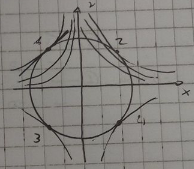
\includegraphics[width=0.3\textwidth]
			{images/IGL1.png}
			\caption{\label{fig:my-label}}}
	\end{figure}	
	Notiamo come graficamente ricaviamo 4 punti critici.
	Se applichiamo lagrange troviamo
	\begin{align}
		{}&\double{\det \matrixTwoTwo{y}{x}{2x}{2y}=0}{x^2 + y^2 =1} \implies \double{x^2 = y^2}{2y^2=1}\nextpassage &\vecx^{1,2,3,4}=(\pm \sqrt{2} \spacecomma\pm \sqrt{2})
	\end{align}
	E quindi abbiamo quattro punti critici anche qui.
	\item $f(x,y)=x+y \spacer g(x,y)=x + y^2 -1$
	\begin{figure}[!htb]
		\center{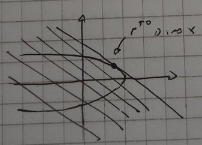
\includegraphics[width=0.3\textwidth]
			{images/IGL2.png}
			\caption{\label{fig:my-label}}}
	\end{figure}
	
	
	In questo caso abbiamo solo un punto di massimo, non essendoci altri punti di tangenza. 
\end{enumerate}

\newpage

\subsection{Oss. sui punti critici}

\begin{figure}[!htb]
	\center{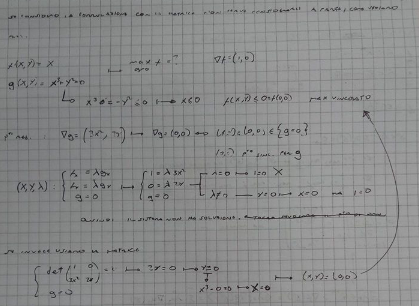
\includegraphics[width=\textwidth]
		{images/soppigro1.png}
		\caption{\label{fig:my-label}}}
\end{figure}

\newpage

\subsection{Metodo dei Moltiplicatori di Lagrange nel caso generale}

\textit{Siano}
\begin{align}
	{}&\deffuncR{n}{} \spacer \deffuncRgen{\vecg}{n}{m} \spacer m<n\\
	&f,\vecg \in C^1(A)
\end{align}
\textit{(Notare come il numero di vincoli deve essere inferiore al numero di variabili.)}

\textit{E sia $\vecx^0 \in A$ tale che}
\begin{enumerate}
	\item $\vecg(\vecx^0)=0$
	\item $\jacobian{g}{\vecx^0}$ \textit{è di rango massimo ($\vecx^0 $ pto regolare per $\vecg$)}
	\item \textit{$\vecx^0 $ punto di ma./min. vincolato di f per $\vecg(\vecx^0)=\veczero_m $}
\end{enumerate}
\textit{Allora avremo di nuovo un risultato esprimibile in tre modi equivalenti:}
\begin{enumerate}
	\item \textit{La matrice}
	\begin{align}
		\veccolFour{\gradient{f}{\vecx^0}}{\gradient{g_1}{\vecx^0}}{\dots}{\gradient{g_m}{\vecx^0}}
	\end{align}
	Sarà di rango massimo.
	\item $\exists \underline{\lambda}^0 \taleche \gradient{f}{\vecx^0} = \braket{\lambda^0 | \gradient{\vecg}{\vecx^0}}=\sum_{j=1}^{m} \lambda^0_j \gradient{g_j}{\vecx^0} $
	\item $\mathcal{L}(\vecx,\underline{\lambda}) = f(\vecx) - \braket{\lambda | \gradient{\vecg}{\vecx^0}} \implies \exists \underline{\lambda}^0 \taleche \gradient{\mathcal{L}}{\vecx^0,\underline{\lambda}^0}=\veczero_n$
\end{enumerate}

Non diamo dimostrazione, ma un paio di esempi operativi nelle prossime pagine.
\newpage
\begin{figure}[!htb]
	\center{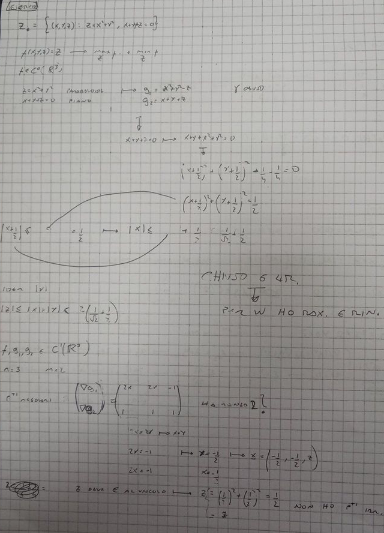
\includegraphics[width=\textwidth]
		{images/esMDL1.png}
		\caption{\label{fig:my-label}}}
\end{figure}

\newpage
\begin{figure}[!htb]
	\center{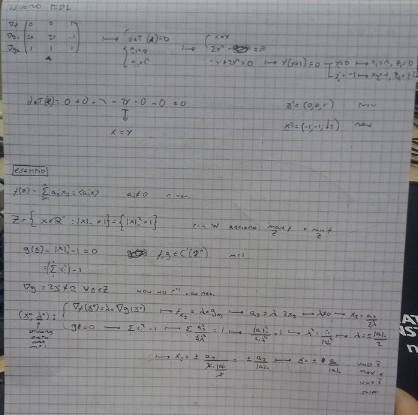
\includegraphics[width=\textwidth]
		{images/esMDL2.png}
		\caption{\label{fig:my-label}}}
\end{figure}
